\section*{第七章}
\begin{center}
{\Large\bfseries 等距适用曲面}
\end{center}
\begin{center}\rule{3em}{0.4pt}\end{center}

\begin{center}\footnotesize
柔性曲面。--高斯关于曲率在弯曲下不变的定理。--判定两个给定曲面能否等距适用的准则。--常曲率曲面的情形。--常曲率曲面的任一部分在同一曲面的任意另一部分上的等距适用性。--容许在自身上连续变形的曲面。--彼此等距适用的旋转曲面。--螺旋面与 Bour 定理。--给定曲面的变形所依赖的二阶偏微分方程。--关于变形的一般定理。--Bonnet 关于保持一个渐近线系而使曲面变形之可能性的定理。
\end{center}

\subsection*{\S. 98.\quad 等距适用曲面。}

在平面几何和球面几何中，人们研究画在平面或球面上的图形的性质，而不考虑它们在空间中的绝对位置；对任意曲面也可以作同样的研究。凡是只涉及画在曲面上的图形之大小与位置关系、并且只把这些图形看作存在于该曲面之上的性质，共同构成\emph{曲面的几何学}。

从这一观点看，形状极不相同的两个曲面可以具有同一种几何学。例如，若把画有图形的平面设想为卷在圆柱面、圆锥面或任意可展曲面上，平面几何的定理显然仍然成立。

为了清楚理解构成曲面几何学的那些性质的本质，可以把曲面设想成一层无限薄、完全柔软而不可伸长的薄膜。

凡在任意弯曲曲面时都不改变的性质，都属于曲面的几何学；其余性质则取决于曲面在空间中的当前形状与位置。

若能在两个曲面 S、S' 的点 P、P' 之间建立一种对应，使对应的线元相等，那么它们具有同一种几何学；因为此时 S 上图形的有限弧长、角与面积，也都等于 S' 上对应图形的相应量。在这种情形下，称两个曲面 S、S' 彼此\emph{等距适用}；这表示只须弯曲其中一个曲面（或它的一部分），便能在不撕裂也不重叠的情况下把它铺展到另一个曲面上。但要把这种铺展看作确实可以实现，显然还须证明存在一族从 S 连续过渡到 S' 的柔性曲面构形。

若已知两个曲面 S、S' 的线元表达式
\[
\begin{aligned}
 ds^2&=E\,du^2+2F\,du\,dv+G\,dv^2,\
 ds'^2&=E'\,du'^2+2F'\,du'\,dv'+G'\,dv'^2,
\end{aligned}
\]
要判定它们是否等距适用，就应考察能否在一个曲面的点 \((u,v)\) 与另一个曲面的点 \((u',v')\) 之间建立一种对应，使线元相等：
\[
 ds=ds'.
\]
因此，两个曲面等距适用的充分必要条件，是微分形式
\[
 E\,du^2+2F\,du\,dv+G\,dv^2
\]
\[
 E'\,du'^2+2F'\,du'\,dv'+G'\,dv'^2
\]
能够相互变换。

由以上论述可知，曲面的几何学已经由它的线元表达式，即第一基本形式，完全确定：
\begin{equation}\tag{1}
 ds^2=E\,du^2+2F\,du\,dv+G\,dv^2.
\end{equation}
换言之，曲面 S 通过弯曲所能呈现的无穷多个构形，具有共同的第一基本形式；其中每一个构形再由其第二基本形式确定（第四章）。

研究由线元确定的曲面几何学时，可以撇开实现这一线元的任何特殊曲面形状。从分析上说，我们得到一个由两个变量 \(u,v\) 生成的二维流形；它的元素（点）由每一组特定值 \((u_0,v_0)\) 给出，这些值属于 \(u,v\)。两个无限邻近点之间的距离 \(ds\)，即点 \((u,v)\) 与 \((u+du,v+dv)\) 之间的距离，按基本定律 (1) 量取；角 \(\theta\) 则是两个线元 \(ds,\delta s\) 之间的角，这两个线元从点 \((u,v)\) 分别连到点 \((u+du,v+dv)\)、\((u+\delta u,v+\delta v)\)，并由公式
\[
 \cos\theta=\frac{E\,du\,\delta u+F(du\,\delta v+dv\,\delta u)+G\,dv\,\delta v}{ds\,\delta s}.
\]
于是，二维流形的点与变量值对 \((u_0v_0)\) 之间存在一一对应。

我们所考虑的 \(u,v\) 变化域总满足如下条件：函数 E、F、G 单值、有限且连续，它们的一阶、二阶偏导数也连续；此外 E、G 和 \(EG-F^2\) 都为正。夹角 \(\omega\) 所属的坐标线为 \(u,v\)，它由公式
\[
 \cos\omega=\frac{F}{\sqrt{EG}},\qquad
 \sen\omega=\frac{\sqrt{EG-F^2}}{\sqrt{EG}},
\]
定义；因此在所考察的区域内，该角在 0 与 \(\pi\) 之间连续变化，而从不取这两个端值。

第二章所讨论的二次形式之不变量与微分参数概念，在这些一般研究中得到直接而重要的应用。曲面的总曲率是形式 (1) 的一个微分不变量；它在每一点的值只依赖于形式 (1) 的系数，所以无论曲面怎样弯曲都保持不变。

由此得到高斯基本定理：\emph{曲面的总曲率在曲面的任何弯曲下都不改变。} 这一结果也可表述为：\emph{若两个曲面等距适用，则它们在两个对应点具有相等的曲率。}

正如前面已经指出的（第134页），正是这一性质使高斯曲率在几何应用中占有首要地位。

现在考察形式 (1) 的一个微分参数，其中含有一个或多个任意函数
\[
 \varphi,
 \qquad \psi\ldots
\]
它在曲面每一点的值与计算时采用的坐标无关，并且在曲面的任意弯曲下保持不变。令 \(\varphi,\psi\ldots\) 分别等于常数，便在曲面上得到相应的若干线系；该微分参数表示这些线所固有的一个量，它不随曲面的弯曲而改变。

例如，考察曲线
\[
 \varphi=\hbox{常数};
\]
的测地曲率 \(\dfrac1{\rho_\varphi}\)。由微分参数（\S.85，第182页）可得
\[
 -\frac1{\rho_\varphi}=\frac{\Delta_2\varphi}{\sqrt{\Delta_1\varphi}}+\nabla\left(\varphi,\frac1{\sqrt{\Delta_1\varphi}}\right).
\]
所以：\emph{曲面上所画曲线的测地曲率，在曲面弯曲时保持不变。}

特别地，曲面 S 的测地线在 S 弯曲后变成新曲面的测地线。这也可以直接从测地线的特征性质（\S.90）看出：在曲面上两个充分邻近的点之间，测地线是最短的曲线。若采用 \S.88（第191页）给出的测地曲率定义，还可由此得到测地曲率在弯曲下不变的另一证明。

还应指出，以上论述也给出了高斯总曲率在弯曲下不变的一个更直观的证明。事实上，取半径为无穷小量 \(u\)、中心为曲面上一点 \(P_0\) 的测地圆；略去高于三阶的无穷小量，其周长 C 由 \S.90 的公式 (15)（第196页）给出：
\[
 C=2\pi u-\frac{\pi K_0u^3}{3},
\]
其中 \(K_0\) 是曲面在 \(P_0\) 处的曲率。无论曲面怎样弯曲，C 的长度不变，因此 \(K_0\) 也不随弯曲而改变。

\subsection*{\S. 99.\quad 第一个等距适用问题的解法。}

利用微分参数理论，可以用最简便的方式解决如下问题：\emph{给定两个曲面 S、S'，判定它们能否彼此等距适用；若能，求出等距适用的公式。}

在分析上，这等价于判定两个给定微分形式
\[
 E\,du^2+2F\,du\,dv+G\,dv^2
\]
\[
 E'\,du'^2+2F'\,du'\,dv'+G'\,dv'^2
\]
能否相互变换。现在设
\begin{equation}\tag{2}
 \begin{cases}
 \varphi(u,v)=\varphi'(u',v'),\\
 \psi(u,v)=\psi'(u',v'),
 \end{cases}
\end{equation}
是 \(u,v,u',v'\) 之间的两个独立关系，并在所假定的等距适用中规定两曲面各点之间的对应。由微分参数的性质，必有
\begin{equation}\tag{3}
 \Delta_1\varphi=\Delta'_1\varphi',
 \qquad
 \nabla(\varphi,\psi)=\nabla'(\varphi',\psi'),
 \qquad
 \Delta_1\psi=\Delta'_1\psi',
\end{equation}
撇号表示右端的微分参数是按第二个形式构造的。因此，等距适用的必要条件是关系 (2) 蕴含关系 (3)。这个必要条件也是充分的。事实上，由 \S.44（第94页）的结果，分别取 \(\varphi,\psi\) 为第一形式的新变量，取 \(\varphi',\psi'\) 为第二形式的新变量，便有
\[
 E\,du^2+2F\,du\,dv+G\,dv^2=
 \frac{\Delta_1\psi\,d\varphi^2-2\nabla(\varphi,\psi)\,d\varphi\,d\psi+\Delta_1\varphi\,d\psi^2}{\Delta_1\varphi\,\Delta_1\psi-\nabla^2(\varphi,\psi)}
\]
\[
 E'\,du'^2+2F'\,du'\,dv'+G'\,dv'^2=
 \frac{\Delta'_1\psi'\,d\varphi'^2-2\nabla'(\varphi',\psi')\,d\varphi'\,d\psi'+\Delta'_1\varphi'\,d\psi'^2}{\Delta'_1\varphi'\,\Delta'_1\psi'-\nabla'^2(\varphi',\psi')}
\]
而由 (2)、(3)，两式右端相等。

在此基础上，先排除两曲面中有一个为常曲率曲面的情形。以 \(K(u,v),K'(u',v')\) 分别表示两曲面的曲率；在等距适用的假设下，高斯定理立即给出一个形如 (2) 的关系：
\begin{equation}\tag{4}
 K(u,v)=K'(u',v').
\end{equation}
此外，K 的任一微分参数显然都应等于 K' 的相应微分参数。先取关系
\begin{equation}\tag{5}
 \Delta_1 K=\Delta'_1 K',
\end{equation}
将它与 (4) 联立，可能出现以下三种情形。

1. \emph{关系 (4)、(5) 相互矛盾}；此时两曲面不能等距适用。

2. \emph{关系 (4)、(5) 相容且彼此独立。} 由上可知，此时两曲面等距适用的充分必要条件，是 (4)、(5) 还蕴含关系
\[
 \nabla(K,\Delta_1 K)=\nabla'(K',\Delta'_1K'),
 \qquad
 \Delta_1(\Delta_1K)=\Delta'_1(\Delta_1K'),
\]
这一点可由代数计算判定。

3. \emph{关系 (4)、(5) 相互归并。}

当 \(\Delta_1K\) 是 K 的函数，而 \(\Delta'_1K'\) 是 K' 的同一函数时，就出现这种情形。

在刚才所考察的情形中，若
\begin{equation}\tag{a}
 \Delta_1K=f(K),
 \qquad
 \Delta'_1K'=f(K'),
\end{equation}
则以另一关系
\begin{equation}\tag{5*}
 \Delta_2K=\Delta'_2K'
\end{equation}
代替 (5)；只要没有进一步出现由下列公式表示的情形，问题便再次化为代数消元：
\begin{equation}\tag{b}
 \Delta_2K=\varphi(K),
 \qquad
 \Delta'_2K'=\varphi(K').
\end{equation}
因此，只剩下 (a)、(b) 同时成立的情形需要考察。

此时
\[
 \frac{\Delta_2K}{\Delta_1K}=\frac{\varphi(K)}{f(K)},
\]
等曲率线 \(K=\) 常数与其正交轨线
\[
 \psi=\hbox{常数},
\]
构成一个等温系统（\S.46，第100页）。

由 \S.47（第100页）的公式，可用求积求得函数 \(\psi(u,v)\)：
\[
\begin{cases}
\displaystyle
 \frac{\partial\psi}{\partial u}=e^{-\int\frac{\varphi(K)}{f(K)}\,dK}
 \frac{F\dfrac{\partial K}{\partial u}-E\dfrac{\partial K}{\partial v}}{\sqrt{EG-F^2}},\\[2.2ex]
\displaystyle
 \frac{\partial\psi}{\partial v}=e^{-\int\frac{\varphi(K)}{f(K)}\,dK}
 \frac{G\dfrac{\partial K}{\partial u}-F\dfrac{\partial K}{\partial v}}{\sqrt{EG-F^2}},
\end{cases}
\]
从而
\[
 \Delta_1\psi=e^{-2\int\frac{\varphi(K)}{f(K)}\,dK}\,\Delta_1K
\]
因此
\[
\begin{aligned}
 E\,du^2+2F\,du\,dv+G\,dv^2
 &=\frac{dK^2}{\Delta_1K}+
 e^{2\int\frac{\varphi(K)}{f(K)}\,dK}\frac{d\psi^2}{\Delta_1K}\\
 &=\frac{dK^2}{f(K)}+
 e^{2\int\frac{\varphi(K)}{f(K)}\,dK}\frac{d\psi^2}{f(K)}.
\end{aligned}
\]
对于第二个曲面，函数 \(f,\varphi\) 保持不变，所以它也具有同样的线元形式；而这一线元形式还属于某个旋转曲面。

所以：\emph{若关系 (a)、(b) 成立，则两个曲面都等距适用于同一个旋转曲面，因而彼此以一个单参数族的方式等距适用。}

如上所见，在这种情形下求出实际的等距适用公式，需要作两次求积。

\subsection*{\S. 100.\quad 常曲率曲面的情形。}

在前两节对第一个等距适用问题的解答中，我们排除了两曲面之一为常曲率曲面的情形。此时，两曲面若要等距适用，另一个曲面也必须具有同一常曲率。值得注意的是，在这种情形下，高斯定理所给的准则也是等距适用的充分条件；即：

\emph{具有同一常曲率的两个曲面彼此等距适用。}

这个定理只是 \S.36（第75页）所证命题的一个特例。具有同一常曲率的两个二元二次微分形式，确实能以一个三参数族的方式相互变换。

对于零曲率曲面，我们在 \S.63（第135页）还从另一途径证明过这一结果，并在那里看出这类曲面是可展曲面。这里将给出一种新证明；它很容易推广到非零常曲率曲面，并且还能为常曲率曲面的线元给出若干确定的典范形式。

在常曲率 K 的曲面上画一条测地线 L，并取与 L 正交的测地线及其正交轨线为坐标线。以参数 \(u\) 表示测地线 \(v\) 的弧长，从 L 起算，因而 L 就是 \(u=0\)；再以 L 上从一个固定点起算的弧长为参数 \(v\)。线元便取形式
\[
 ds^2=du^2+G\,dv^2
\]
由于曲线 \(u=0\) 的测地曲率为零，故
\begin{equation}\tag{\mbox{\(\alpha\)}}
 \left(\frac{\partial\sqrt G}{\partial u}\right)_{u=0}=0
\end{equation}
又因为 \(u=0\) 上的弧长微元正是 \(dv\)，所以
\begin{equation}\tag{\mbox{\(\beta\)}}
 \left(\sqrt G\right)_{u=0}=1.
\end{equation}
现在我们有
\begin{equation}\tag{\mbox{\(\gamma\)}}
 K=-\frac1{\sqrt G}\frac{\partial^2\sqrt G}{\partial u^2};
\end{equation}
按假设 K 为常数；区分三种情形
\[
 K=0,
 \qquad K>0,
 \qquad K<0,
\]
便得到如下结果。

1. 若 \(K=0\)，则
\[
 \sqrt G=\varphi(v)\,u+\psi(v),
\]
其中 \(\varphi(v),\psi(v)\) 是 \(v\) 的函数。但由 \((\alpha),(\beta)\) 得
\[
 \varphi(v)=0,
 \qquad \psi(v)=1,
\]
从而
\[
 ds^2=du^2+dv^2,
\]
这就是平面的线元。

2. 若 \(K>0\)，令
\[
 K=\frac1{R^2}\quad (\hbox{R 为实数}),
\]
由 \((\gamma)\) 得
\[
 \sqrt G=\varphi(v)\cos\frac{u}{R}+\psi(v)\sen\frac{u}{R},
\]
再由 \((\alpha),(\beta)\) 得
\[
 \psi(v)=0,
 \qquad \varphi(v)=1,
\]
所以
\begin{equation}\tag{6}
 ds^2=du^2+\cos^2\left(\frac{u}{R}\right)dv^2.
\end{equation}
这个线元属于半径为 R 的球面；因此：

\emph{一切具有正的常曲率 \(\dfrac1{R^2}\) 的曲面，都等距适用于半径为 R 的球面，因而也彼此等距适用。}

3. 若 \(K<0\)，令
\[
 K=-\frac1{R^2}
\]
则 \((\gamma)\) 给出
\[
 \sqrt G=\varphi(v)\cosh\frac{u}{R}+\psi(v)\senh\frac{u}{R},
\]
再由 \((\alpha),(\beta)\) 得
\[
 \varphi(v)=1,
 \qquad \psi(v)=0.
\]
所以：\emph{半径为 R 的任意伪球面的线元都能化为形式}
\begin{equation}\tag{7}
 ds^2=du^2+\cosh^2\left(\frac{u}{R}\right)dv^2.
\end{equation}
由此可见，所有这些曲面都彼此等距适用。

\subsection*{\S. 101.\quad 常曲率曲面在自身上的 \(\infty^3\) 个等距适用。}

以上结果也可用于同一常曲率曲面的两个部分，而不只是用于具有同一常曲率的两个不同曲面；于是得到重要定理：

\emph{常曲率曲面的任一部分都能等距适用于同一曲面的任意另一部分；并且，只要 A' 到 B' 的测地距离等于 A 到 B 的测地距离，就能使第一部分的任意两点 A、B 分别与第二部分的任意两点 A'、B' 重合。}

对于零或正常曲率曲面，该定理显然成立，因为它们分别等距适用的平面和球面正具有上述性质。为对伪球面也作严格证明，先把上一节中的测地线 L 取为 AB，于是
\[
 ds^2=du^2+\cosh^2\frac{u}{R}\,dv^2,
\]
其中沿 AB 的弧长参数 \(v\) 从 A 起算，故 \(A\equiv(0,0)\)。对第二条测地线 A'B' 作同样处理，得到
\[
 ds'^2=du'^2+\cosh^2\frac{u'}{R}\,dv'^2.
\]
现在只须令
\[
 u'=u,
 \qquad v'=v,
\]
便有
\[
 ds^2=ds'^2
\]
点 \(A\equiv(0,0)\) 对应于 \(A'\equiv(0,0)\)，点 \(B\equiv(0,l)\) 对应于 \(B'\equiv(0,l)\)，其中 \(l\) 是弧 AB、A'B' 的共同长度。因此，该曲面能以 A 与 A'、B 与 B' 分别重合的方式等距适用于自身，正如所断言的。

这个定理说明，画在常曲率曲面上的任一图形，都能只通过弯曲移到该曲面的任意另一部分，而角、长度与面积都不发生改变。

所以，对于常曲率曲面的几何学，像对于平面和球面一样，一般都成立\emph{图形可叠合原理}。正如后文将见，这是三类曲面几何学之间诸多类比的基础。

由高斯定理还可立即看出，这一原理对任何其他曲面都不成立。

由以上论述可知，具有同一常曲率的两个曲面 S、S'，彼此有一个三参数族的等距适用。给定两曲面，要找出其中一种等距适用方式，就须积分\emph{测地线方程}。若曲率为零，问题可用求积解决（\S\S.15、93）；在其余情形中，问题归结为\emph{积分一个 Riccati 型一阶微分方程}，这一点将在另一章证明（见第十三章，\S.182）。

\subsection*{\S. 102.\quad 伪球面 \(ds^2\) 的三种典型形式。}

现在回到线元的形式 (7)，它适用于任意半径为 R 的伪球面。这种线元形式称为\emph{双曲型}；此外还要考察另外两种同样重要的线元形式，分别称为\emph{椭圆型}和\emph{抛物型}。

取伪球面上的一个普通点 P，以从 P 发出的测地线 \(v\) 及其正交轨线 \(u\) 为坐标线；以该测地线束中的动测地线与一条固定测地线的夹角为参数 \(v\)，并以从 P 起算的测地线弧长为参数 \(u\)。线元便取形式
\[
 ds^2=du^2+G\,dv^2
\]
并且（\S.90）
\[
 \left(\sqrt G\right)_{u=0}=0,
 \qquad
 \left(\frac{\partial\sqrt G}{\partial u}\right)_{u=0}=1.
\]
由 \S.100 已知
\[
 \sqrt G=\varphi(v)\cosh\frac{u}{R}+\psi(v)\senh\frac{u}{R}
\]
上述条件给出
\[
 \varphi(v)=0,
 \qquad \psi(v)=R,
\]
从而
\[
 ds^2=du^2+R^2\senh^2\frac{u}{R}\,dv^2.
\]
这是适用于每个半径为 R 的伪球面的线元形式，称为\emph{椭圆型}。

最后，把 \S.100 中的曲线 L 不取为测地线，而取为测地曲率恒为 \(\dfrac1R\) 的曲线。半径为 R 的伪球面上的这种曲线称为\emph{极限圆}\srcfn{1}{不难看出，每一个伪球面上都有一个双参数族的极限圆；这些性质将在另一章作更详细的研究。}。仍有
\[
 ds^2=du^2+G\,dv^2,
 \qquad
 \sqrt G=\varphi(v)\cosh\frac{u}{R}+\psi(v)\senh\frac{u}{R}
\]
而且必须满足
\[
 \left(\sqrt G\right)_{u=0}=1,
 \qquad
 \left(\frac1{\sqrt G}\frac{\partial\sqrt G}{\partial u}\right)_{u=0}
 =\frac1R\left[\frac{\varphi(v)\senh\dfrac{u}{R}+\psi(v)\cosh\dfrac{u}{R}}{\varphi(v)\cosh\dfrac{u}{R}+\psi(v)\senh\dfrac{u}{R}}\right]_{u=0}=\frac1R,
\]
由此得到
\[
 \varphi(v)=\psi(v)=1,
\]
从而
\[
 ds^2=du^2+e^{\frac{2u}{R}}\,dv^2.
\]
第三种形式称为\emph{抛物型}。

综上，对于半径为 R 的伪球面，我们得到线元的三种典型形式：
\[
 \hbox{A) 抛物型：}\quad ds^2=du^2+e^{\frac{2u}{R}}dv^2
\]
\[
 \hbox{B) 椭圆型：}\quad ds^2=du^2+R^2\senh^2\left(\frac{u}{R}\right)dv^2
\]
\[
 \hbox{C) 双曲型：}\quad ds^2=du^2+\cosh^2\left(\frac{u}{R}\right)dv^2.
\]

\subsection*{\S. 103.\quad 伪球旋转面。}

现在考察最简单的一类伪球面，即旋转面。

以子午线和平行线为坐标线时，它们的线元具有如下形式（第221页）：
\[
 ds^2=du^2+\left(Ce^{\frac{u}{R}}+C'e^{-\frac{u}{R}}\right)^2dv^2.
\]
按两个常数 C、C' 中有一个为零、二者异号或二者同号，分成三种情形。把参数 \(v\) 换成 \(cv_1\)（\(c\) 为常数），分别得到 A)、B)、C) 三型的形式
\[
\begin{aligned}
\hbox{I)}\quad &ds^2=du^2+e^{\frac{2u}{R}}dv_1^2,\\
\hbox{II)}\quad &ds^2=du^2+\lambda^2\senh^2\frac{u}{R}\,dv_1^2,\\
\hbox{III)}\quad &ds^2=du^2+\lambda^2\cosh^2\frac{u}{R}\,dv_1^2,
\end{aligned}
\]
其中 \(\lambda\) 为常数。用三个旋转面实现这些线元，使 \(u\) 为子午线弧长、\(v_1\) 为经度。以 \(r\) 表示平行圆半径，以 \(z=\varphi(r)\) 表示子午曲线方程，则三种情形分别为
\[
\begin{aligned}
\hbox{I)}\quad &r=e^{\frac{u}{R}},
& z&=\int\sqrt{1-\frac1{R^2}e^{\frac{2u}{R}}}\,du,\\[0.8ex]
\hbox{II)}\quad &r=\lambda\senh\frac{u}{R},
& z&=\int\sqrt{1-\frac{\lambda^2}{R^2}\cosh^2\left(\frac{u}{R}\right)}\,du,\\[0.8ex]
\hbox{III)}\quad &r=\lambda\cosh\frac{u}{R},
& z&=\int\sqrt{1-\frac{\lambda^2}{R^2}\senh^2\left(\frac{u}{R}\right)}\,du.
\end{aligned}
\]
下面讨论三条子午曲线的形状。

在情形 I) 中，可以用初等函数完成积分。令
\[
 e^{\frac{u}{R}}=R\sen\varphi,
\]
则 \(\varphi\) 是子午曲线切线与 \(z\) 轴的夹角，而公式
\[
 r=R\sen\varphi,
 \qquad
 z=R\int\frac{\cos^2\varphi}{\sen\varphi}\,d\varphi
 =R\left\{\log\tg\frac12\varphi+\cos\varphi\right\}
\]
给出曲线上一点的坐标，以 \(\varphi\) 为参数。

这些方程所表示的曲线以 \(z\) 轴为渐近线，并具有如下性质：它的切线在切点与渐近线之间所截的一段恒等于 R；这条曲线称为\emph{曳物线}。这一性质既可直接从曲线方程验证，也可由相应旋转面之平行圆的测地曲率恒等于 \(\dfrac1R\) 推出（参见第224页）。该旋转面称为\emph{伪球面}，是伪球面的最简单形态\srcfn{1}{本图及以下两图取自达姆施塔特 L. \textsc{Brill} 制作的模型目录。}。

\begin{center}
\begin{minipage}{0.45\linewidth}
\centering
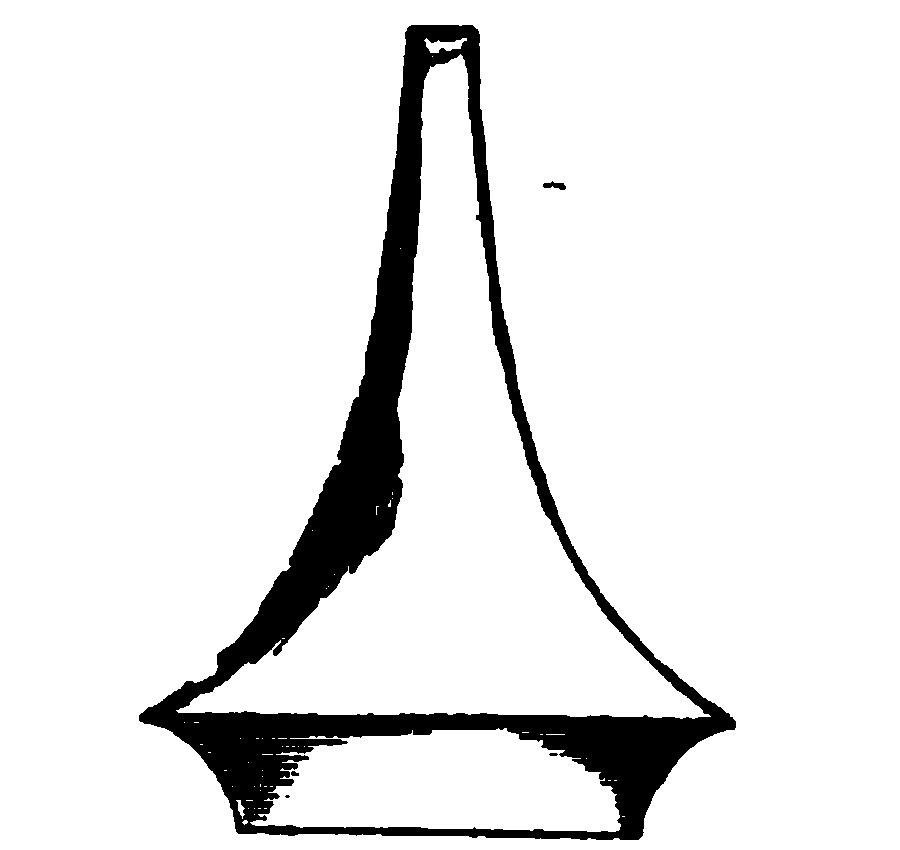
\includegraphics[width=0.82\linewidth]{assets/ch07_figures/F1_EMBED_DETERMINISTIC_GRAY8.png}\\[-.2em]
{\footnotesize\bfseries 图1.\({}^{\rm a}\)--伪球面。}
\end{minipage}
\end{center}

\emph{情形 II：椭圆型。} 为得到实曲面，必须假设
\[
 \frac{\lambda}{R}<1
\]
令 \(\lambda=R\sen\alpha\)，则 \(\cosh\dfrac{u}{R}\) 的最大值为 \(\dfrac1{\sen\alpha}\)，所以平行圆半径 \(r\) 在
\[
 r=0
 \qquad\hbox{e}\qquad
 r=R\cos\alpha.
\]
当 \(r=0\) 时，\(\dfrac{dr}{du}=\sen\alpha\)；因此所有子午线都在 \(u=0\) 处以角 \(\alpha\) 与旋转轴相交，这一点是曲面的锥点。

子午曲线上一点的坐标可表示为参数 \(\tau\) 的椭圆函数，其模为 \(k=\cos\alpha\)。事实上，令
\[
 \senh\frac{u}{R}=\frac{k}{k'}\cn(\tau,k)
\]
便有
\[
 r=Rk\cn\tau,
 \qquad
 z=Rk'\int_0^\tau \sn^2\tau\,d\tau
 =R\left\{\frac{H}{K}\tau-Z(\tau)\right\},
\]
其中
\[
 Z(\tau)=\frac{\Theta'(\tau)}{\Theta(\tau)}
\]
是 Jacobi 函数，H、K 是椭圆函数理论中的熟知常数。曲线上从 \(\tau=0\) 到 \(\tau=2K\) 的一段绘于图 II)；当 \(\tau\) 增加 \(4K\) 时，曲线周期性重复。相应的旋转面由沿轴平移后全等的无穷多个部分组成；半径 \(r=R\cos\alpha\) 的最大平行圆是曲面的回归线，因为 \(\tau=2mK\)（\(m\) 为整数）处是子午曲线的尖点。

\begin{center}
\begin{minipage}{0.55\linewidth}
\centering
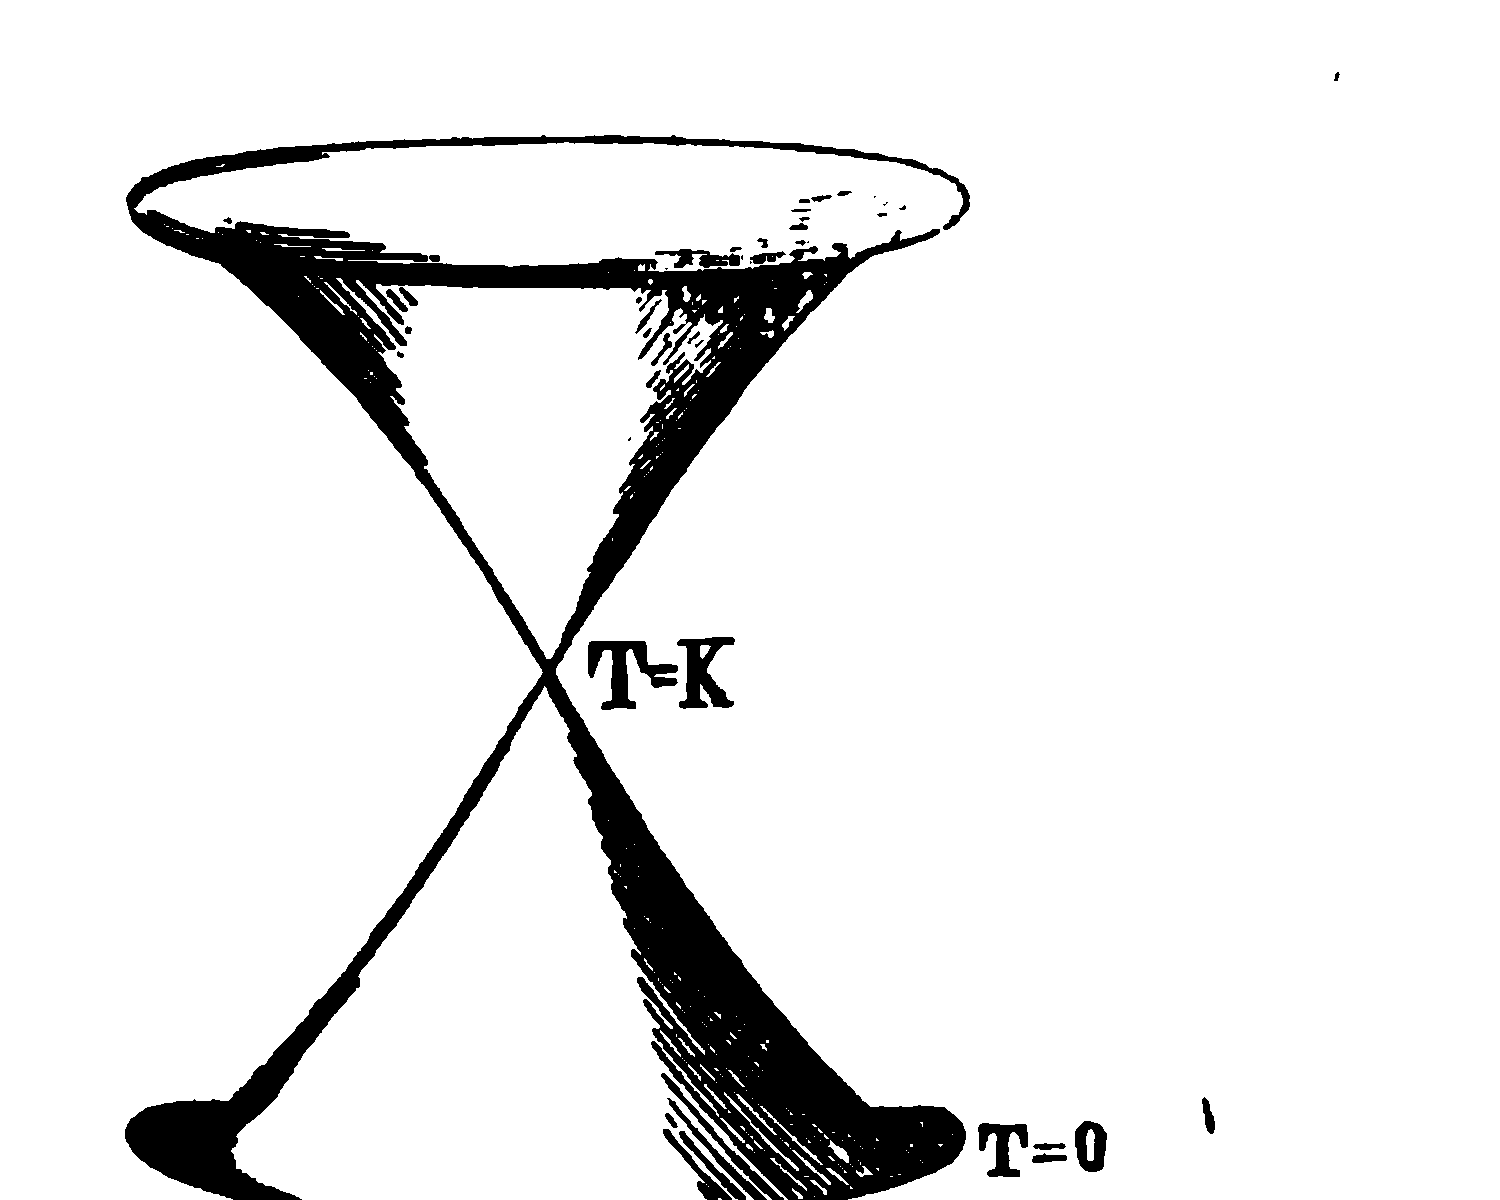
\includegraphics[width=0.96\linewidth]{assets/ch07_figures/F2_EMBED_DETERMINISTIC_GRAY8.png}\\[-.2em]
{\footnotesize\bfseries 图2.\({}^{\rm a}\)--椭圆型伪球旋转面。}
\end{minipage}
\end{center}

\emph{情形 III：双曲型。} 此时
\[
 r=\lambda\cosh\frac{u}{R},
 \qquad
 \frac{dr}{du}=\frac{\lambda}{R}\senh\frac{u}{R};
\]
曲线实部中 \(u\) 的最大值对应于 \(\senh\dfrac{u}{R}=\dfrac{R}{\lambda}\)，而平行圆半径在最小值 \(\lambda\) 与最大值 \(\sqrt{R^2+\lambda^2}\) 之间变化。

令
\[
 \frac{R}{\sqrt{R^2+\lambda^2}}=k,
 \qquad
 \cosh\frac{u}{R}=\frac{\dn(\tau,k)}{k},
\]
则曲线上动点的坐标可由参数 \(\tau\) 的椭圆函数表示为
\[
 r=\frac{R}{k}\dn\tau,
 \qquad
 z=\frac{R}{k}\left\{\frac{H}{K}\tau-Z(\tau)\right\}.
\]
从 \(\tau=0\) 到 \(\tau=2K\) 的曲线形状绘于图3.\({}^{\rm a}\)；当 \(\tau\) 增加 \(2K\) 时，曲线周期性重复。对应于 \(\tau=2mK\)（\(m\) 为整数）的最大平行圆是曲面的回归线，而对应于 \(\tau=(2m+1)K\) 的最小平行圆是测地线。

\begin{center}
\begin{minipage}{0.48\linewidth}
\centering
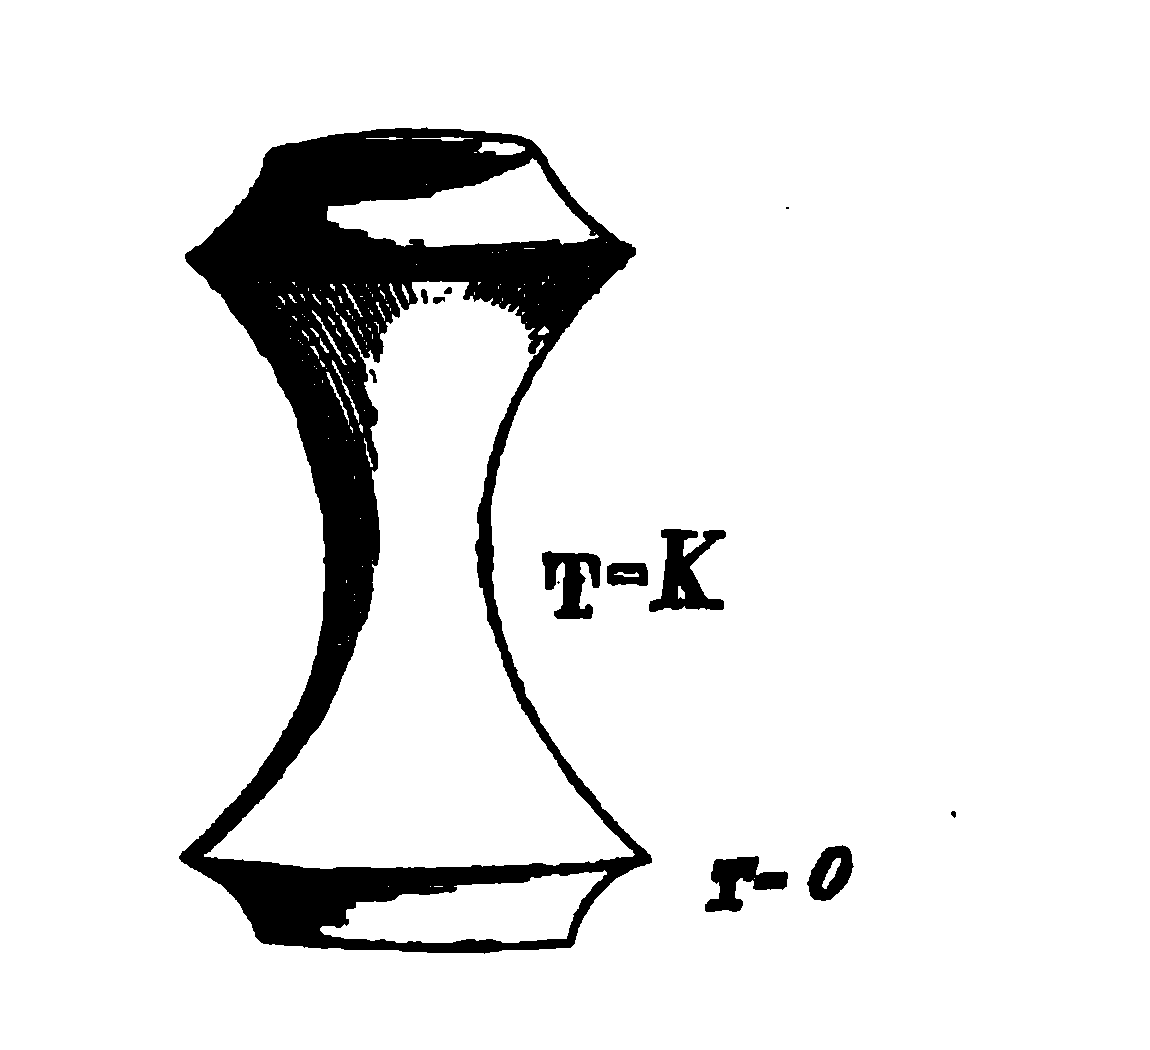
\includegraphics[width=0.85\linewidth]{assets/ch07_figures/F3_EMBED_DETERMINISTIC_GRAY8.png}\\[-.2em]
{\footnotesize\bfseries 图3.\({}^{\rm a}\)--双曲型伪球旋转面。}
\end{minipage}
\end{center}

以上三种伪球旋转面彼此不同；也不可能把其中一种等距适用于另一种不同类型的曲面，同时使平行圆仍铺展到平行圆上。只须注意：抛物型中平行圆的测地曲率恒为 \(\dfrac1R\)，椭圆型中为 \(>\dfrac1R\)，而双曲型中为 \(<\dfrac1R\)，即可判明这一点。不过由一般定理（\S.100），任一半径为 R 的伪球面都能等距适用于 I)、II)、III) 中的每一个曲面。为更仔细说明任一伪球面变形为旋转面的方式，作如下观察：

a) 在伪球面 S 上画一条极限圆，并考察与它正交的测地线。通过弯曲，可使该曲面成为伪球面，而所画测地线变成子午线。

b) 在伪球面 S 上标出一点 P，考察从 P 发出的测地线及其正交的测地圆。按第224页选取参数 \(u,v\)，便有
\[
 ds_1^2=du^2+R^2\senh^2\frac{u}{R}\,dv^2.
\]
与椭圆型旋转面的线元
\[
 ds_1^2=du_1^2+\lambda^2\senh^2\frac{u_1}{R}\,dv_1^2,
\]
比较，得到等距适用公式
\[
 u_1=u,
 \qquad
 \frac{\lambda}{R}v_1=v.
\]
由此可见，当旋转面 II) 上的经度 \(v_1\) 从 0 到 \(2\pi\) 转过一整圈时，角 \(v\) 只遍历从 \(v=0\) 到 \(v=2\pi\sen\alpha<2\pi\) 的区间。因此，S 上 P 附近的一部分就足以完全覆盖曲面 II) 的一叶。此外，S 上位于半径为
\[
 u=\sett\cosh\left(\frac1{\sen\alpha}\right)
\]
的测地圆之外的部分，在曲面 II) 上没有对应点；因而 S 上可变形成曲面 II) 一叶的 P 邻域，由一个测地扇形界定。

c) 对于双曲型曲面 III)，最小平行圆是一条测地线；因此可把任一伪球面 S 等距适用于 III)，使 S 的任意测地线 \(g\) 铺展到该最小平行圆上。S 上实际铺到 III) 一叶上的部分，是一个带状区域：其两侧由两条与 \(g\) 测地平行且到它等距的曲线界定，这两条曲线变形后成为该叶的最大平行圆（回归线）；沿测地线 \(g\) 的方向，该带又由两条与 \(g\) 正交的测地线界定，它们变形后合并为该叶的一条子午线。带的长度和宽度只取决于拟赋予最小平行圆的半径。

\subsection*{\S. 104.\quad 容许在自身上作 \(\infty^1\) 个等距适用的曲面。}

在 \S.100 证明的常曲率曲面之基本性质，可以表述为：

\emph{任一常曲率曲面的线元都容许一个 \(\infty^3\) 的自身变换族。}

现在问：是否还有别的曲面容许在自身上作连续弯曲？若这种弯曲构成一个双参数族，那么利用变换的两个参数，可以把曲面的每一点移到（某一适当区域内的）任意另一点；由高斯定理，该曲面必有常曲率，而所假定的弯曲就应构成三参数族，而不是双参数族。

显然，任何等距适用于某一旋转面的曲面，都容许在自身上作连续弯曲；这种弯曲对应于该旋转面绕轴的旋转。

重要的是，逆定理也成立：

\emph{凡容许在自身上作连续弯曲的曲面 S，都等距适用于某一旋转面。} 这一点实质上已由 \S.99 的讨论得到，因为那里看出：两个曲面 S、S' 的等距适用公式只有在它们都等距适用于同一旋转面时，才能含有一个任意参数。不过也可由以下几何论证重新证明。若 S 具有常曲率，前几节已经证明该定理；否则，在所假定的连续弯曲中，等曲率线 L
\[
 K=\hbox{常数}
\]
由高斯定理必沿自身滑动。由于这种弯曲依赖于一个连续变化的参数，L 上任一点都能移到 L 上任意另一点；所以 L 具有常测地曲率。此外，与某条 L 测地平行的各条曲线，在上述弯曲中也显然沿自身滑动。由此容易推出所述定理；事实上成立如下性质：

\emph{若曲面 S 具有一个由测地平行且测地曲率为常数的曲线 L 组成的线系，那么 S 等距适用于某一旋转面，而该旋转面的平行圆正是曲线 L 的变形。}

事实上，取曲线 L（\(u=\) 常数）及其正交测地线（\(v=\) 常数）组成的坐标系；线元成为
\[
 ds^2=du^2+G\,dv^2.
\]
按假设有
\[
 -\frac1{\rho_u}=\frac{\partial\log\sqrt G}{\partial u}=\varphi(u),
\]
所以
\[
 \sqrt G=UV,
\]
其中 U 只是 \(u\) 的函数，V 只是 \(v\) 的函数。令
\[
 \int V\,dv=v_1,
\]
便显出线元
\[
 ds^2=du^2+U^2\,dv_1^2
\]
属于一个旋转面。

\subsection*{\S. 105.\quad 彼此等距适用的旋转面。}

现在考察一些等距适用曲面的简单例子。首先研究两个旋转面 S、S\(_1\) 能否彼此等距适用。

首先由高斯定理，S 的平行圆必铺展到 S\(_1\) 的平行圆上，因而子午线也铺展到子午线上。常曲率曲面当然是例外；但若附加一个曲面的平行圆铺到另一个曲面平行圆上的条件，以下论证对它们也成立。

若 S 的线元为
\[
 ds^2=du^2+r^2\,dv^2
\]
而 S\(_1\) 的线元为
\[
 ds_1^2=du_1^2+r_1^2\,dv_1^2,
\]
从两个对应平行圆起算子午线弧长，便可直接令 \(u_1=u\)。为使两个线元相互变换，令 \(v_1=v_1(v)\)，并由条件
\[
 r_1(u)\frac{dv_1}{dv}=r(u).
\]
确定该函数。由此得
\[
 r_1=kr,
 \qquad
 v_1=\frac{v}{k}\quad (k\hbox{ 为任意常数}).
\]
因此，若 \(r=\varphi(u)\) 是 S 的子午曲线方程，则 S\(_1\) 的子午曲线坐标为
\[
 r=k\varphi(u),
 \qquad
 z=\int\sqrt{1-k^2\varphi'^2(u)}\,du.
\]
所以：\emph{每个旋转面都能以一个 \(\infty^1\) 的方式族变形，同时仍保持为旋转面。}

再仔细考察 S\(_1\) 等距适用于 S 的方式。若设 \(k<1\)，公式
\[
 v=kv_1
\]
表明：当经度 \(v_1\) 在 S\(_1\) 上转过一整圈而成为 \(2\pi\) 时，经度 \(v\) 变为
\[
 v=2k\pi<2\pi.
\]
所以把 S\(_1\) 铺到 S 上时，S 不会被完全覆盖；两条子午线之间会留下一个扇形部分，其所在平面的夹角为 \(2\pi(1-k)\)。要把 S\(_1\) 铺展到 S 上，必须先沿一条子午线切开 S\(_1\)，再把它张开并变形，使切口的两条边在 S 上成为两条不同的子午线。注意平行圆的测地曲率和曲面的总曲率在变形中不变，立即可知：在对应点上，S 的子午曲线曲率大于 S\(_1\) 的子午曲线曲率。

情形 \(k>1\) 显然对应于 S 到 S\(_1\) 的逆变形：须从 S 去掉一个扇形，再把被去掉扇形的两条子午线通过变形合成一条，以恢复曲面的连续性。还应注意，S 子午曲线上的一点在 S\(_1\) 的子午曲线上有实对应点，只要 \(k\dfrac{dr}{du}<1\)；当 \(k<1\) 时这总是成立。但当 \(k>1\) 时，对应于 \(\dfrac1k\) 这个 \(\dfrac{dr}{du}\) 值的平行圆在 S 上界定出一个带状区域，这才是 S 中实际能等距适用于 S\(_1\) 的部分。变形后，该带的两个边界平行圆成为 S\(_1\) 的回归平行圆。

作为例子，考察常曲率旋转面的变形。

a) 对半径为\emph{一}的球面，可取
\[
 r=\cos u
\]
变形后的子午曲线坐标为
\[
 r=k\cos u,
 \qquad
 z=\int\sqrt{1-k^2\sen^2 u}\,du.
\]
可把它们表示为参数 \(\tau\) 的椭圆函数。若 \(k<1\)，令 \(\cos u=\cn(\tau,k)\)，则
\[
 r=k\cn\tau,
 \qquad
 z=\left(1-\frac{H}{K}\right)\tau+Z(\tau);
\]
若 \(k>1\)，把 \(k\) 换成 \(\dfrac1k\)，并令
\[
 \cos u=\dn(\tau,k)
\]
则
\[
 r=\frac{\dn\tau}{k},
 \qquad
 z=\left(k-\frac{H}{Kk}\right)\tau+\frac1k Z(\tau).
\]
当 \(k<1\) 时，得到一个纺锤形曲面，其子午线以角 \(\alpha=\arc\sen k\) 在一点与轴相交；该点是曲面的锥点。当 \(k>1\) 时，得到一个由两个最小回归平行圆界定的带状区域。以下三图分别表示这三种情形所对应的曲面；在中间的球面上，标出了能等距适用于图6.\({}^{\rm a}\) 曲面的区域。

\begin{center}
\begin{minipage}[t]{0.29\linewidth}
\centering
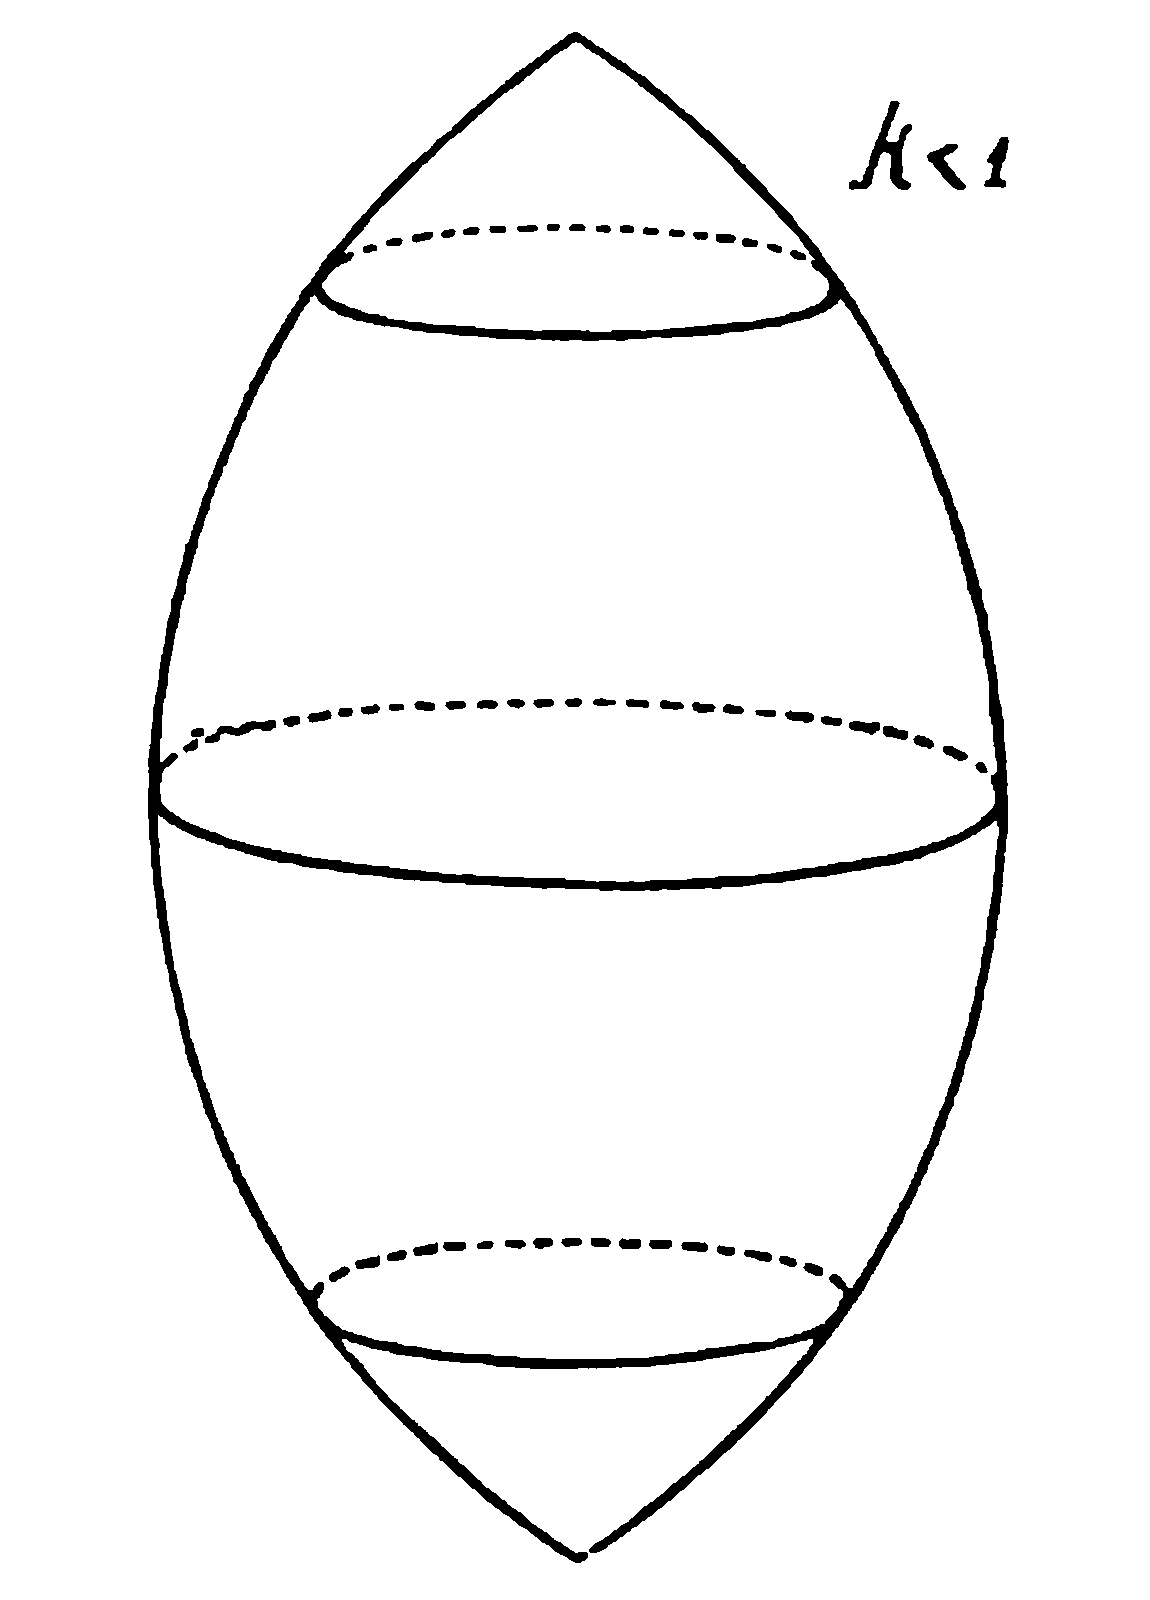
\includegraphics[width=0.92\linewidth]{assets/ch07_figures/F4_EMBED_DETERMINISTIC_GRAY8.png}\\[-.2em]
{\footnotesize\bfseries 图4.\({}^{\rm a}\)}
\end{minipage}\hfill
\begin{minipage}[t]{0.37\linewidth}
\centering
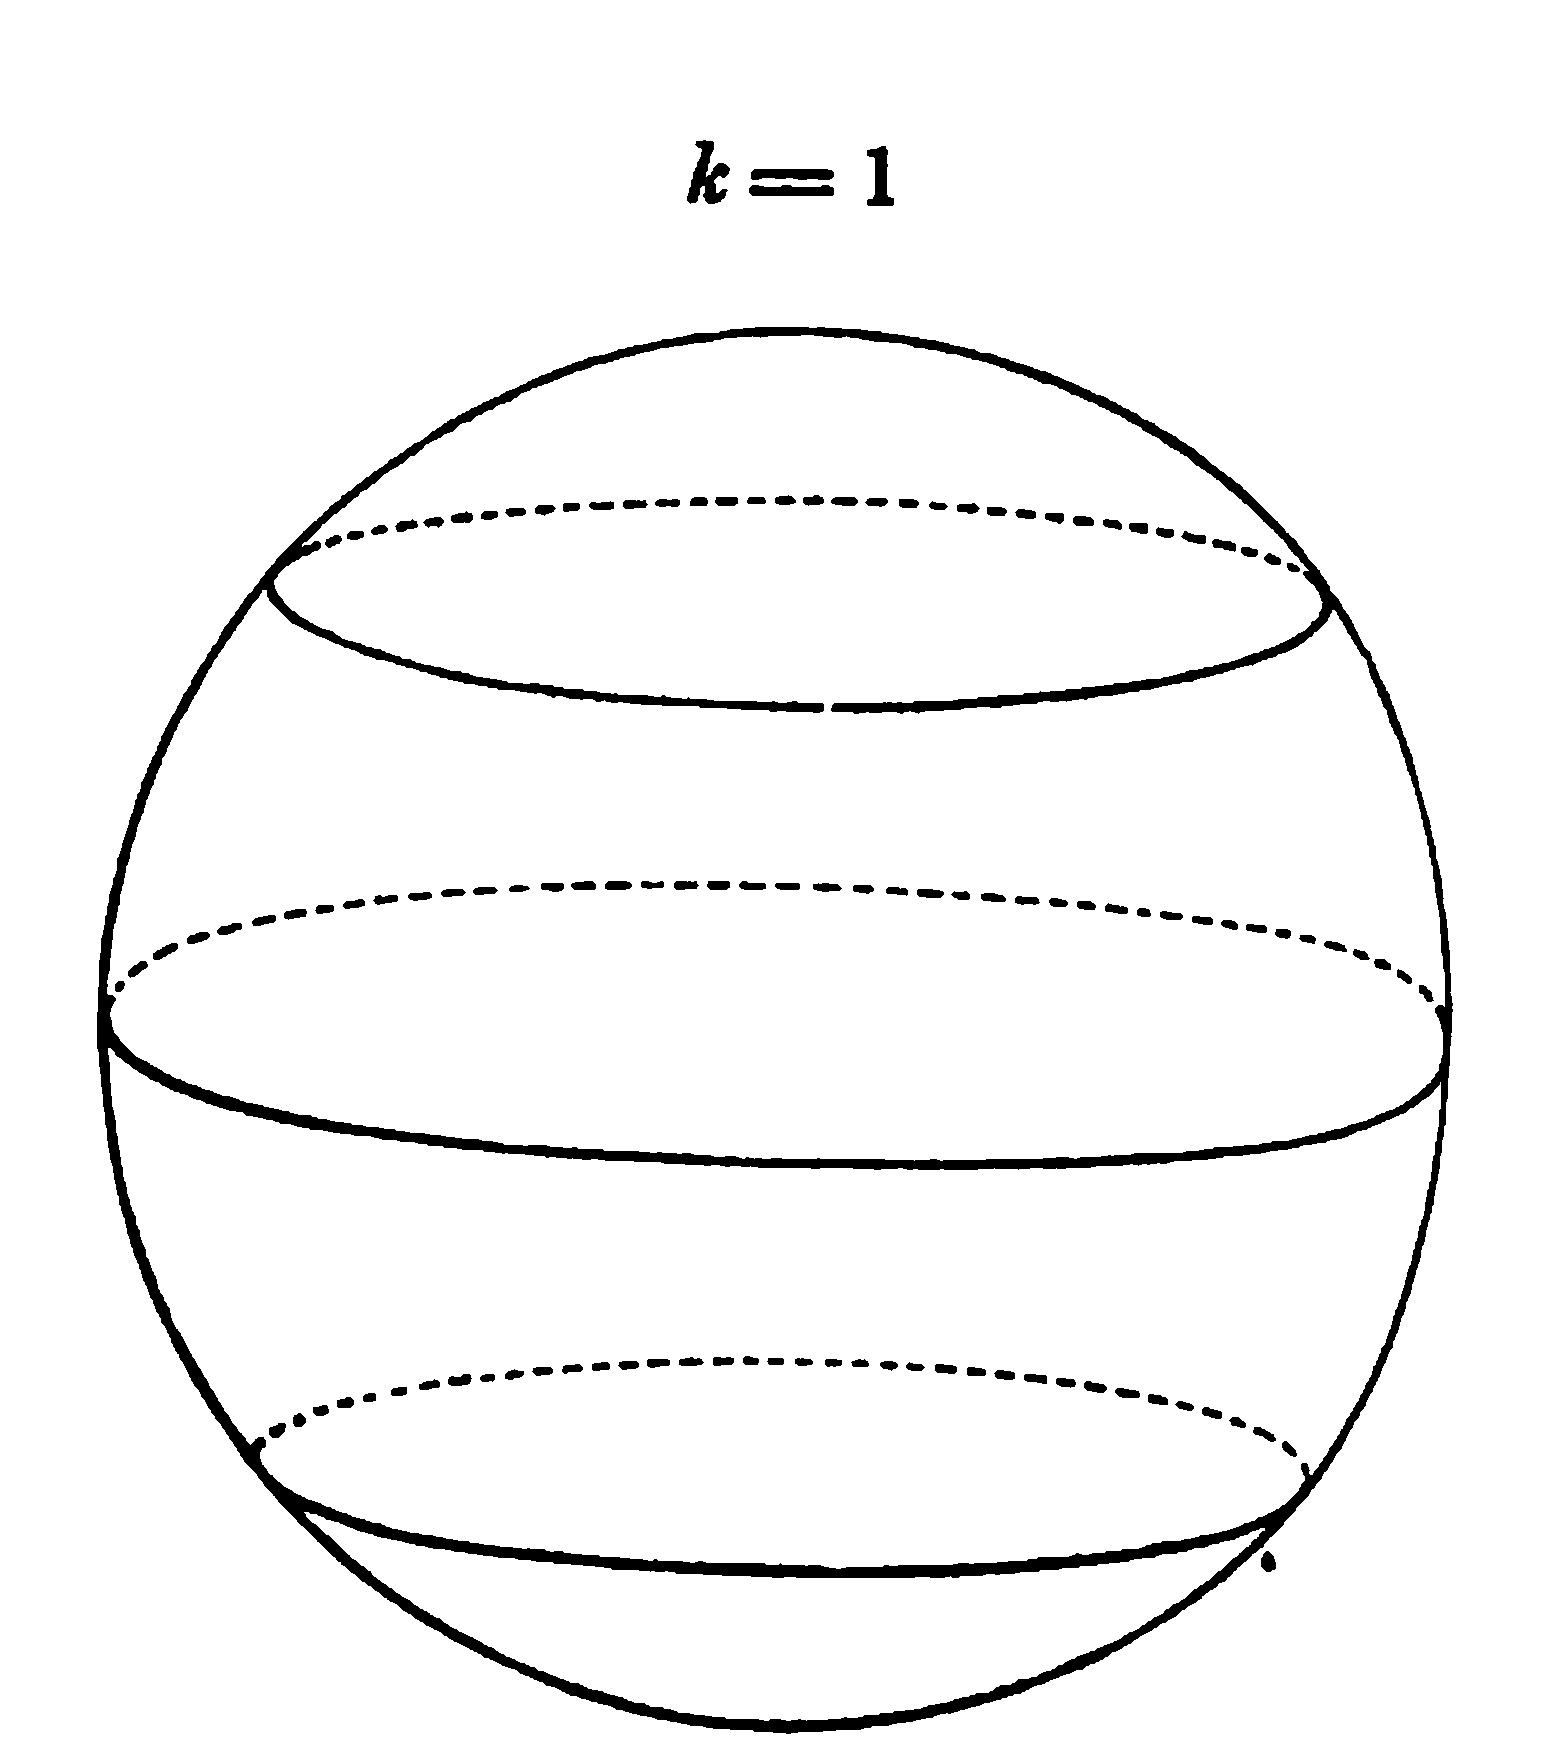
\includegraphics[width=0.98\linewidth]{assets/ch07_figures/F5_EMBED_DETERMINISTIC_GRAY8.png}\\[-.2em]
{\footnotesize\bfseries 图5.\({}^{\rm a}\)--（球面）。}
\end{minipage}

\medskip
\begin{minipage}{0.48\linewidth}
\centering
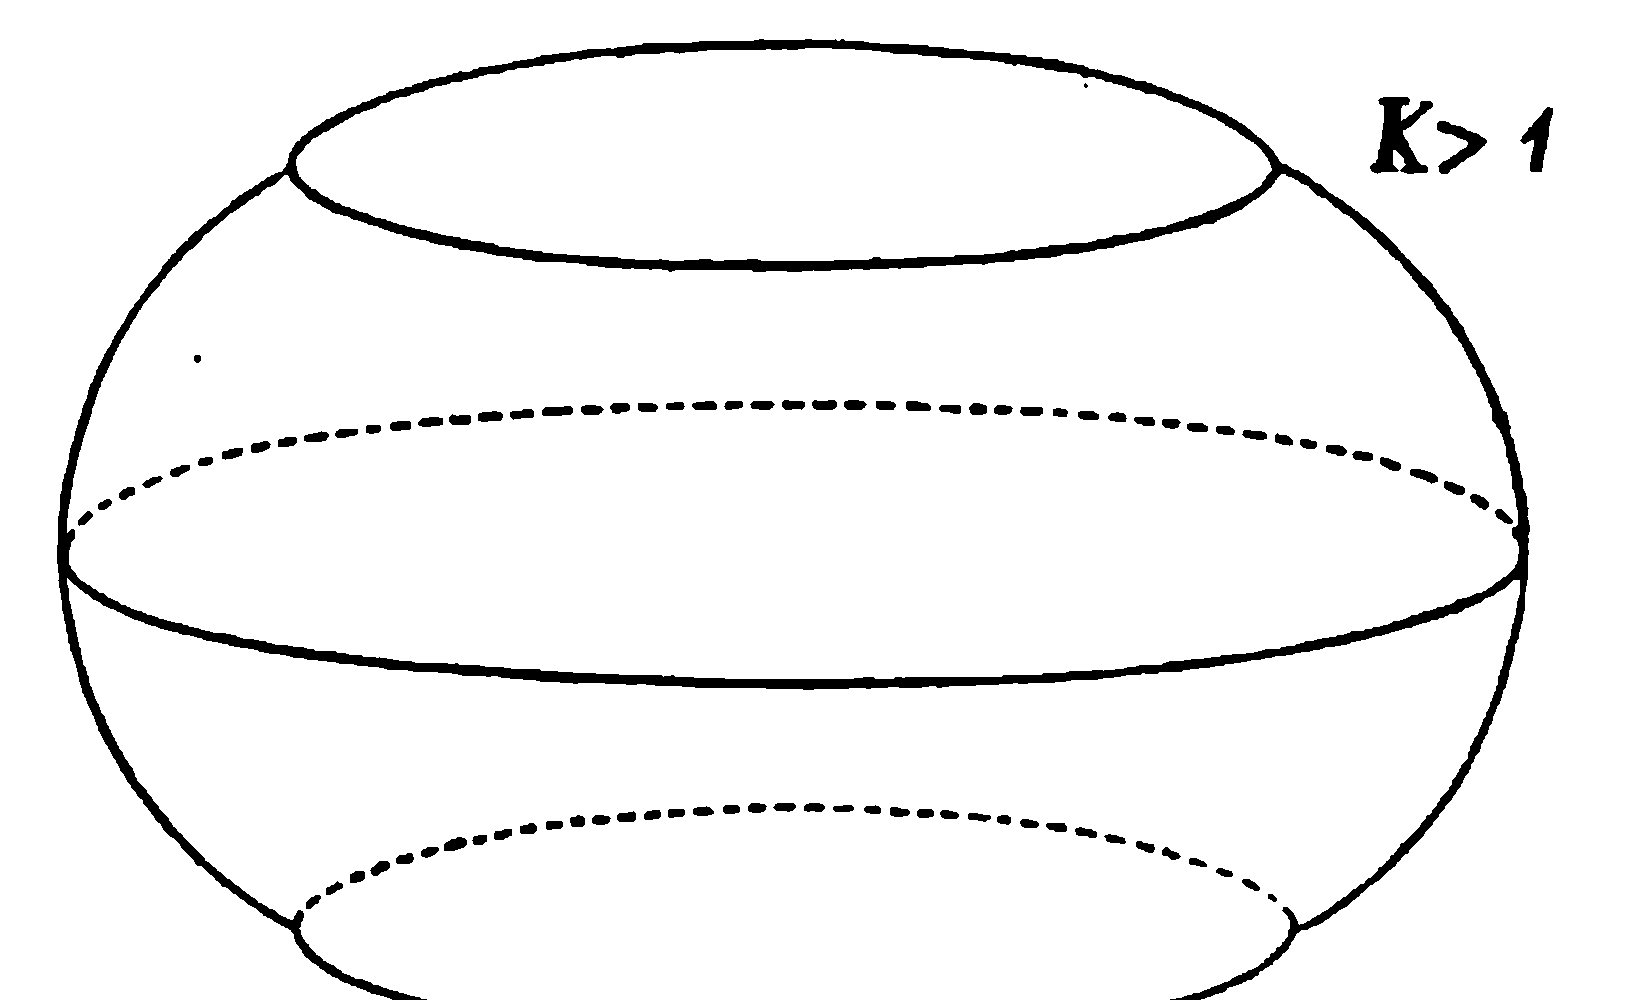
\includegraphics[width=0.98\linewidth]{assets/ch07_figures/F6_EMBED_DETERMINISTIC_GRAY8.png}\\[-.2em]
{\footnotesize\bfseries 图6.}
\end{minipage}
\end{center}

b) 伪球面具有一个特殊性质：它的所有旋转变形都与伪球面本身重合。这由平行圆的测地曲率恒 \(=\dfrac1R\) 立即可见。

在平行圆收缩的情形（\(k<1\)）中，最大平行圆（回归线）变成一个较小的平行圆，因而该平行圆与最大平行圆之间的带状区域未被覆盖。在逆变形中，一个较小的平行圆变成回归平行圆；但要实现这种变形，必须先从伪球面上切去该平行圆与现有回归平行圆之间的区域。

另外两类伪球旋转面的变形仍得到同类型的曲面：椭圆型中改变顶点（锥点）的张角，双曲型中改变最小平行圆的半径。

\subsection*{\S. 106.\quad 螺旋面与 Bour 定理。}

\S.104 的结果可立即应用于一类重要曲面，称为\emph{螺旋面}。这类曲面由一条平面曲线或空间曲线生成：曲线一面绕某轴旋转，一面沿该轴平移，而且两种运动的速度之比为常数。母线的各点分别描出圆螺线，它们以螺旋面的轴为共同轴，并具有同一螺距。生成曲面的螺旋运动使整个曲面沿自身滑动；应用 \S.105 的定理，便得到 Bour 的优美结果：

\emph{每个螺旋面都等距适用于一个旋转面；螺线铺展为平行圆。}

显然，该旋转面被螺旋面覆盖无穷多次，因为每条螺线都绕相应的平行圆无穷多圈。

现在直接证明该定理，同时求出实际的等距适用公式。过轴作一平面，它在螺旋面上截出一条曲线；若使这条截线（\emph{子午剖线}）作生成该曲面的螺旋运动，它便描出整个螺旋面。给定子午剖线和螺旋运动的参数，螺旋面就完全确定。

取螺旋面的轴为 \(z\) 轴，以 \(\rho\) 表示子午剖线上一点到该轴的距离，设
\[
 z=\varphi(\rho)
\]
为子午剖线的方程。再以 \(v\) 表示经过任意时间后子午剖面所转过的角，以 \(m\) 表示平移速度与旋转速度之比。螺旋面上动点的坐标 \(x,y,z\) 作为 \(\rho,v\) 的函数为
\[
 x=\rho\cos v,
 \qquad y=\rho\sen v,
 \qquad z=\varphi(\rho)+mv,
\]
从中
\[
 ds^2=\{1+\varphi'^2(\rho)\}\,d\rho^2+2m\varphi'(\rho)\,d\rho\,dv+(\rho^2+m^2)\,dv^2.
\]
变换坐标线 \(v\)，令
\[
 v=kv_1-m\int\frac{\varphi'(\rho)\,d\rho}{\rho^2+m^2},
\]
其中 \(k\) 为任意常数；于是
\[
 ds^2=\left\{1+\frac{\rho^2\varphi'^2(\rho)}{\rho^2+m^2}\right\}d\rho^2+k^2(\rho^2+m^2)\,dv_1^2.
\]
把这个线元与旋转面的线元
\[
 ds_1^2=\{1+\psi'^2(r)\}\,dr^2+r^2dv_1^2
\]
相比较；其中
\[
 z=\psi(r)
\]
是子午曲线方程。若令 \(r,\psi(r),\rho,\varphi(\rho)\) 满足关系
\begin{equation}\tag{8}
\left\{
\begin{aligned}
 r^2&=k^2(\rho^2+m^2),\\
 \{1+\psi'^2(r)\}\left(\frac{dr}{d\rho}\right)^2
 &=1+\frac{\rho^2\varphi'^2(\rho)}{\rho^2+m^2}.
\end{aligned}
\right.
\end{equation}
便能使两个线元相同。这些公式再次证明 Bour 定理；而且还表明：任取一个螺旋面或一个旋转面，都可用求积找出与之等距适用的旋转面或螺旋面。第一种情形中消去 \(\rho\)，便得到 \(\psi'(r)\)；第二种情形中消去 \(r\)，便得到 \(\varphi'(\rho)\)。

\subsection*{\S. 107.\quad 极小直纹螺旋面与单叶双曲面。}

把公式 (8) 应用于两个简单例子。

1. 子午剖线是一条垂直于轴的直线；所生成的螺旋面就是第一章 \S.24 已考察的\emph{极小直纹螺旋面}。此时 (8) 中 \(\varphi'(\rho)=0\)，所以
\[
 1+\psi'^2(r)=\left(\frac{d\rho}{dr}\right)^2=\frac{r^2}{k^2(r^2-m^2k^2)}
\]
取任意常数 \(k=1\)，得到
\[
 z=\psi(r)=m\int\frac{dr}{\sqrt{r^2-m^2}}
\]
作此求积便有
\[
 r=m\cosh\frac{z}{m}.
\]
所以子午曲线是一条普通悬链线，其准线为旋转轴。

相应的旋转面称为\emph{悬链面}。螺旋面的直母线铺展到子午线上，而轴 \(\rho=0\) 变成悬链面的腰圆 \(r=m\)。

2. 子午剖线是一条与轴成角 \(\alpha\) 的直线；其方程为
\[
 z=\rho\cot\alpha
\]
把
\[
 \varphi'(\rho)=\cot\alpha,
\]
代入 (8)，得到
\[
 1+\psi'^2(r)=\left\{1+\frac{(r^2-k^2m^2)\cot^2\alpha}{r^2}\right\}
 \frac{r^2}{k^2(r^2-k^2m^2)}
\]
再令
\[
 k=\cot\alpha,
\]
便有
\[
 \psi'(r)=\frac{\tg\alpha\,r}{\sqrt{r^2-m^2\cot^2\alpha}}.
\]
所以旋转面的子午曲线方程为
\[
 z=\tg\alpha\sqrt{r^2-m^2\cot^2\alpha},
\]
即
\[
 \frac{r^2}{m^2\cot^2\alpha}-\frac{z^2}{m^2}=1.
\]
因此，该旋转面是单叶旋转双曲面。容易看出，螺旋面的轴 \(\rho=0\) 铺展到双曲面的腰圆上，而螺旋面的直母线铺展到双曲面一个直母线系的母线上。

\subsection*{\S. 108.\quad 第二个等距适用问题。}

现在转向等距适用理论的第二个、也是更重要的问题：\emph{求出所有等距适用于给定曲面的曲面}，或者说：\emph{求出具有给定线元的所有曲面}。

这个困难问题只有在少数特殊情形中知道如何完全解决；后文将考察这些情形。不过，偏微分方程的一般定理使我们能建立一些关于该问题的极重要的一般结果。现在就在本书篇幅所容许的范围内讨论这些结果\srcfn{1}{读者可在 Darboux《讲义》第三卷第263页及以下找到这个问题的完整论述。}。

处理这一问题的第一种方法自然来自曲面论的基本公式（第四章）。给定第一基本形式
\[
 E\,du^2+2F\,du\,dv+G\,dv^2,
\]
每一个具有此线元的曲面都对应一个第二基本形式
\[
 D\,du^2+2D'\,du\,dv+D''\,dv^2,
\]
函数 \(D,D',D''\) 必须满足 \S.56（第119页）的方程 (III)、(IV)，即高斯方程与两个 Codazzi 方程。反过来，若 \(D,D',D''\) 是满足这三个方程的 \(u,v\) 的函数，就存在一个具有给定线元的对应曲面；实际求出该曲面还须解一个 Riccati 方程。

例如，若取旋转面的线元
\[
 ds^2=du^2+r^2dv^2,
\]
就可令 \(D,D',D''\) 只为 \(u\) 的函数来满足上述基本方程。这样得到的等距适用于旋转面的曲面，恰是 \S.106 的螺旋面\srcfn{1}{为证明这一点，只须注意此时第一、第二基本形式都容许连续的自身变换
\[
 u'=u,\qquad v'=v+\hbox{常数}
\]
因此曲面容许在自身上的连续运动，故为螺旋面。}。

\subsection*{\S. 109.\quad 第二个问题的偏微分方程。}

比前一种方法更重要的是下面的方法；它以 \S.69 所得结果，确切地说以第146页方程 (B) 为基础。

对于任一曲面
\[
 x=x(u,v),\qquad y=y(u,v),\qquad z=z(u,v)
\]
若其给定线元为
\begin{equation}\tag{9}
 dx^2+dy^2+dz^2=E\,du^2+2F\,du\,dv+G\,dv^2
\end{equation}
上述方程表明，三个未知函数 \(x,y,z\) 中的每一个都满足二阶偏微分方程
\begin{equation}\tag{10}
 \Delta_{22}x=(1-\Delta_1x)K,
\end{equation}
其系数正由 \(E,F,G\) 及其一阶、二阶导数构成\srcfn{2}{采用 Monge 记号，以 \(p,q;r,s,t\) 表示未知函数的一阶、二阶导数，方程写成
\[
\begin{aligned}
&\left(r-\chr{1}{1}{1}p-\chr{1}{1}{2}q\right)
 \left(t-\chr{2}{2}{1}p-\chr{2}{2}{2}q\right)
-\left(s-\chr{1}{2}{1}p-\chr{1}{2}{2}q\right)^2 \\
&\hspace{3em}=K\left\{EG-F^2-\left[E q^2-2Fpq+G p^2\right]\right\}
\end{aligned}
\]
它关于 \(rt-s^2\) 及 \(r,s,t\) 具有 Ampère 线性形式。}。

现在应随 Darboux 指出，方程 (10) 具有如下意义：
\begin{center}
\emph{若 \(x(u,v)\) 是它的一个解，则二次形式}
\end{center}
\[
\begin{aligned}
&E\,du^2+2F\,du\,dv+G\,dv^2-dx^2 \\
&=\left\{E-\left(\frac{\partial x}{\partial u}\right)^2\right\}du^2
+2\left\{F-\frac{\partial x}{\partial u}\frac{\partial x}{\partial v}\right\}du\,dv
+\left\{G-\left(\frac{\partial x}{\partial v}\right)^2\right\}dv^2
\end{aligned}
\]
\begin{center}
\emph{具有零曲率。}\end{center}
为以最简方式证明，令
\[
 x=u,
 \qquad F=0,
\]
由方程的不变性，这显然是允许的。于是 (10) 变为
\[
 \chr{1}{1}{1}\chr{2}{2}{1}-\chr{1}{2}{1}^2=G(E-1)K
\]
代入 Christoffel 符号在此时的值
\[
 \chr{1}{1}{1}=\frac1{2E}\frac{\partial E}{\partial u},\qquad
 \chr{1}{2}{1}=\frac1{2E}\frac{\partial E}{\partial v},\qquad
 \chr{2}{2}{1}=-\frac1{2E}\frac{\partial G}{\partial u},
\]
得到
\[
 \frac{\partial E}{\partial u}\frac{\partial G}{\partial u}
 +\left(\frac{\partial E}{\partial v}\right)^2
 +4E^2G(E-1)K=0.
\]
现在在正交坐标中我们有（\S.43，第93页）：
\begin{equation}\tag{11}
\begin{aligned}
4E^2G^2K={}&E\left[\frac{\partial E}{\partial v}\frac{\partial G}{\partial v}+
\left(\frac{\partial G}{\partial u}\right)^2\right]
+G\left[\frac{\partial E}{\partial u}\frac{\partial G}{\partial u}+
\left(\frac{\partial E}{\partial v}\right)^2\right]\\
&-2EG\left[\frac{\partial^2E}{\partial v^2}+\frac{\partial^2G}{\partial u^2}\right]
\end{aligned}
\end{equation}
前一方程乘以 \(G\)，可写成
\[
\begin{aligned}
&G\left[\frac{\partial E}{\partial u}\frac{\partial G}{\partial u}+
\left(\frac{\partial E}{\partial v}\right)^2\right]
+E(E-1)\left[\frac{\partial E}{\partial v}\frac{\partial G}{\partial v}+
\left(\frac{\partial G}{\partial u}\right)^2\right] \\
&\quad+G(E-1)\left[\frac{\partial E}{\partial u}\frac{\partial G}{\partial u}+
\left(\frac{\partial E}{\partial v}\right)^2\right]
-2EG(E-1)\left(\frac{\partial^2E}{\partial v^2}+\frac{\partial^2G}{\partial u^2}\right)=0.
\end{aligned}
\]
消去相互抵消的项并除以 \(E\)，得到等价方程
\[
\begin{aligned}
&(E-1)\left[\frac{\partial E}{\partial v}\frac{\partial G}{\partial v}+
\left(\frac{\partial G}{\partial u}\right)^2\right]
+G\left[\frac{\partial G}{\partial u}\frac{\partial E}{\partial u}+
\left(\frac{\partial E}{\partial v}\right)^2\right]\\
&\qquad -2(E-1)G\left[\frac{\partial^2E}{\partial v^2}+\frac{\partial^2G}{\partial u^2}\right]=0,
\end{aligned}
\]
由 (11) 可知，它恰好表示形式
\[
 (E-1)du^2+Gdv^2
\]
具有零曲率。

在此基础上，设已知方程 (10) 的一个解 \(x(u,v)\)，考察是否存在具有给定线元的对应实曲面。微分形式
\begin{equation}\tag{12}
 E\,du^2+2F\,du\,dv+G\,dv^2-dx^2
\end{equation}
此时具有零曲率。要存在另外两个满足 (9) 的实函数 \(y(u,v),z(u,v)\)，充分必要条件是 (12) 为正定形式，即
\[
\left[E-\left(\frac{\partial x}{\partial u}\right)^2\right]
\left[G-\left(\frac{\partial x}{\partial v}\right)^2\right]
-\left[F-\frac{\partial x}{\partial u}\frac{\partial x}{\partial v}\right]^2>0,
\]
即
\[
 \Delta_1x<1.
\]
若此条件满足，则可用求积求出 \(y,z\)（\S\S.37、93）；显然，\(y,z\) 只差一个坐标变换而确定。

所以：\emph{方程 (10) 的每一个实解 \(x(u,v)\)，若还满足不等式 \(\Delta_1x<1\)，都对应一个且仅一个具有给定线元的实曲面。已知该解后，对应曲面可由求积得到。}

\subsection*{\S. 110.\quad 含有一条刚性曲线时曲面的不可变形性。}

现在考察如下问题：\emph{给定曲面 S 及画在其上的曲线 \(\Gamma\)，能否弯曲该曲面而不使这条曲线变形？}

假设可以，并以 \(S_1\) 表示 S 在弯曲后保持 \(\Gamma\) 刚性不变的一种形状。可设 \(S_1\) 与初始形状充分接近，使 \(S_1\)、S 沿 \(\Gamma\) 的法线任意接近。又因 \(\Gamma\) 在 \(S_1\) 与 S 上具有同一测地曲率，并由测地曲率与绝对曲率的关系（\S.84），立即得出：沿 \(\Gamma\)，\(S_1\) 与 S 的法线重合。

为简单起见，在 S（以及 \(S_1\)）上取正交坐标系 \((u,v)\)，令
\[
 v=0
\]
为曲线 \(\Gamma\) 的方程。以附加下标 1 表示与 \(S_1\) 有关的量，显然有
\[
\left.
\begin{gathered}
 x_1=x,
 \quad y_1=y,
 \quad z_1=z,\\
 \frac{\partial x_1}{\partial u}=\frac{\partial x}{\partial u},\quad
 \frac{\partial y_1}{\partial u}=\frac{\partial y}{\partial u},\quad
 \frac{\partial z_1}{\partial u}=\frac{\partial z}{\partial u},\\
 \frac{\partial x_1}{\partial v}=\frac{\partial x}{\partial v},\quad
 \frac{\partial y_1}{\partial v}=\frac{\partial y}{\partial v},\quad
 \frac{\partial z_1}{\partial v}=\frac{\partial z}{\partial v},\\
 X_1=X,
 \quad Y_1=Y,
 \quad Z_1=Z
\end{gathered}
\right\}\quad \hbox{当 }v=0.
\]
例如考察 \(x_1,x\)：它们是同一个二阶偏微分方程 (10) 的解，并且在 \(v=0\) 上函数值及一阶导数值都相同。若能证明\emph{\(x_1\) 的三个二阶导数也分别等于 \(x\) 的对应二阶导数（在 \(v=0\) 上）}，那么由偏微分方程解的一般定理\srcfn{1}{例如参见 \textsc{Goursat}，\emph{Leçons sur l'intégration des équations aux dérivées partielles du premier ordre}，第22页。}，即可断定 \(x_1,x\) 对一切 \(u,v\) 都相同。对 \(y_1,y;z_1,z\) 重复同一论证，便得到 \(S_1,S\) 重合。由初始条件
\[
 \frac{\partial x_1}{\partial u}=\frac{\partial x}{\partial u},
 \qquad
 \frac{\partial x_1}{\partial v}=\frac{\partial x}{\partial v},
 \quad \hbox{当 }v=0
\]
首先推出
\[
 \frac{\partial^2x_1}{\partial u^2}=\frac{\partial^2x}{\partial u^2},
 \qquad
 \frac{\partial^2x_1}{\partial u\partial v}=\frac{\partial^2x}{\partial u\partial v},
 \quad \hbox{当 }v=0.
\]
于是曲面论的基本公式 (I)（\S.55，第116页）给出
\[
 D_1=D,
 \qquad D'_1=D',
 \quad \hbox{当 }v=0.
\]
等式
\[
 DD''-D'^2=D_1D''_1-D_1'^2,
\]
在 \(v=0\) 上给出
\[
 DD''=DD''_1,
 \quad \hbox{当 }v=0.
\]
因此
\[
 (D''_1)_{v=0}=(D'')_{v=0},
\]
\emph{除非} \((D)_{v=0}=0\)。排除这一情形，由上述 \S.55 公式 (I) 的第三式，正好得到所要证明的
\[
 \frac{\partial^2x_1}{\partial v^2}=\frac{\partial^2x}{\partial v^2},
 \quad \hbox{当 }v=0,
\]
因而 \(S_1,S\) 重合。

在被排除的情形 \((D)_{v=0}=0\) 中，曲线 \(v=0\) 是 S 的渐近线。因此可陈述定理：\emph{若柔性曲面 S 上的一条曲线 \(\Gamma\) 保持刚性，则曲面不能变形；唯一可能的例外是 \(\Gamma\) 为 S 的一条渐近线。}

若 \(\Gamma\) 是渐近线，偏微分方程的进一步性质（这里只能略加指出）表明确实可以在不使该曲线变形的情况下变形曲面。这是渐近线的一个特殊性质，因此渐近线也称为\emph{折线}。它区别于曲面上其他一切曲线，根本原因是：任一曲面 S 的渐近线，正是决定 S 变形的偏微分方程 (10) 的\emph{特征线}\srcfn{1}{把 (10) 写成上一节注中的形式
\[
 \Phi(r,s,t)=0
\]
则特征线的微分方程
\[
 \frac{\partial\Phi}{\partial t}\,du^2-\frac{\partial\Phi}{\partial s}\,du\,dv+\frac{\partial\Phi}{\partial r}\,dv^2=0,
\]
由 \S.55 的公式 (I)，恰变为渐近线的微分方程
\[
 D\,du^2+2D'\,du\,dv+D''\,dv^2=0
\]
（参见\textsc{Darboux}，t.III，第 252 页）。}。

\subsection*{\S. 111.\quad 指定一条曲线变形后形状的曲面变形。}

刚才证明的定理自然引出如下问题：\emph{能否使曲面 \(S'\) 变形，使其上一条指定曲线 C 取得预先给定的形状 \(\Gamma\)？}

首先注意：若所求变形存在，则 \(\Gamma\) 在每一点的绝对曲率必须大于或等于 C 在对应点的测地曲率。设此条件满足；暂且还排除 \(\Gamma\) 的绝对曲率与测地曲率相等的情形，因为那时 \(\Gamma\) 将是变形后曲面上的渐近线。

假设所求变形存在，以 S 表示变形后的曲面。在 S 上像上一节那样取正交坐标系 \((u,v)\)，使曲线 \(\Gamma\) 为 \(v=0\)。为明确起见，再规定参数 \(u\) 是从 \(\Gamma\) 上一固定点起算的弧长，于是
\[
 E=1,
 \quad \hbox{当 }v=0.
\]
以 \(\sigma\) 表示如下有向角：在 \(\Gamma\) 的法平面内，把 S 的正法线方向沿正向转到 \(\Gamma\) 的主法线方向所需转过的角。对曲线 \(\Gamma\) 仍采用曲线论（第一章）的通常记号，则在 \(v=0\) 上有
\begin{equation}\tag{13}
\left\{
\begin{aligned}
\alpha&=\frac{\partial x}{\partial u},
&\beta&=\frac{\partial y}{\partial u},
&\gamma&=\frac{\partial z}{\partial u},\\
\xi&=\cos\sigma\,X-\sen\sigma\,\frac1{\sqrt G}\frac{\partial x}{\partial v},
&\eta&=\cos\sigma\,Y-\sen\sigma\,\frac1{\sqrt G}\frac{\partial y}{\partial v},\\
\zeta&=\cos\sigma\,Z-\sen\sigma\,\frac1{\sqrt G}\frac{\partial z}{\partial v},\\
\lambda&=-\cos\sigma\,\frac1{\sqrt G}\frac{\partial x}{\partial v}-\sen\sigma\,X,
&\mu&=-\cos\sigma\,\frac1{\sqrt G}\frac{\partial y}{\partial v}-\sen\sigma\,Y,\\
\nu&=-\cos\sigma\,\frac1{\sqrt G}\frac{\partial z}{\partial v}-\sen\sigma\,Z.
\end{aligned}
\right.
\end{equation}
又有
\[
 \frac{\partial^2x}{\partial u^2}=\chr{1}{1}{1}\frac{\partial x}{\partial u}+
 \chr{1}{1}{2}\frac{\partial x}{\partial v}+DX=\frac{\xi}{\rho}
\]
以及关于 \(y,z\) 的类似公式；并且由于
\begin{equation}\tag{14}
 \chr{1}{1}{1}_{v=0}=\left(\frac1{2E}\frac{\partial E}{\partial u}\right)_{v=0}=0,
 \qquad
 \chr{1}{1}{2}_{v=0}=-\frac1{2G}\frac{\partial E}{\partial v}=\left(\frac1{\rho_v}\right)_{v=0}-\frac1{\sqrt G},
\end{equation}
与 (13) 比较得到
\begin{equation}\tag{15}
 D=\frac{\cos\sigma}{\rho},
 \qquad
 \frac1{\rho_v}=-\frac{\sen\sigma}{\rho}.
\end{equation}
第二式中，绝对曲率 \(\dfrac1\rho\) 与测地曲率 \(\dfrac1{\rho_v}\) 属于 \(\Gamma\) 且都已知，因而给出未知角 \(\sigma\) 的两个互补值。

取 \(\sigma\) 的这两个值之一；每个值事实上都导向一个相应曲面 S\srcfn{1}{因而本问题有两个不同解，这并不与 \S.110 的定理矛盾。如此得到的两个曲面 S 的确彼此等距适用；在一个曲面连续变形为另一个曲面的过程中，曲线 \(\Gamma\) 最终恢复初始形状，但在中间状态会改变形状。}。由 (13)，在 \(v=0\) 上，\(\dfrac{\partial x}{\partial v},\dfrac{\partial y}{\partial v},\dfrac{\partial z}{\partial v}\) 的初值为
\begin{equation}\tag{16}
\left\{
\begin{aligned}
\frac{\partial x}{\partial v}&=-\sqrt G(\xi\sen\sigma+\lambda\cos\sigma),\\
\frac{\partial y}{\partial v}&=-\sqrt G(\eta\sen\sigma+\mu\cos\sigma),\\
\frac{\partial z}{\partial v}&=-\sqrt G(\zeta\sen\sigma+\nu\cos\sigma).
\end{aligned}
\right.
\end{equation}
还应记下 \(X,Y,Z\) 沿 \(\Gamma\) 的值：
\begin{equation}\tag{11*}
\left\{
\begin{aligned}
X&=\xi\cos\sigma-\lambda\sen\sigma,\\
Y&=\eta\cos\sigma-\mu\sen\sigma,\\
Z&=\zeta\cos\sigma-\nu\sen\sigma.
\end{aligned}
\right.
\end{equation}
由此可知，对方程 (10)
\[
 \Delta_{22}\theta=(1-\Delta_1\theta)K
\]
的这三个解，还知道函数本身以及下列二阶偏导数在 \(v=0\) 上的初值：
\[
 \frac{\partial^2x}{\partial u^2},\quad
 \frac{\partial^2x}{\partial u\partial v},\quad
 \frac{\partial^2y}{\partial u^2},\quad
 \frac{\partial^2y}{\partial u\partial v},\quad
 \frac{\partial^2z}{\partial u^2},\quad
 \frac{\partial^2z}{\partial u\partial v},
\]
它们所满足的偏微分方程 (10)，还会给出\emph{至少其中一个解}的二阶导数
\[
 \frac{\partial^2x}{\partial v^2},\quad
 \frac{\partial^2y}{\partial v^2},\quad
 \frac{\partial^2z}{\partial v^2},
\]
的值；否则，在 \(v=0\) 上，表达式
\[
 \frac{\partial^2x}{\partial u^2}-\chr{1}{1}{1}\frac{\partial x}{\partial u}-\chr{1}{1}{2}\frac{\partial x}{\partial v},
\]
以及关于 \(y,z\) 的两个类似表达式都必须为零。但代入初值并利用 (15) 的第二式，它们分别成为
\[
\frac{\cos\sigma}{\rho}(\xi\cos\sigma-\lambda\sen\sigma),\quad
\frac{\cos\sigma}{\rho}(\eta\cos\sigma-\mu\sen\sigma),\quad
\frac{\cos\sigma}{\rho}(\zeta\cos\sigma-\nu\sen\sigma)
\]
只有在已排除的情形 \(\sigma=\dfrac{\pi}{2}\) 中，它们才会同时为零。因此不失一般性，可设
\[
(\alpha)\qquad \xi\cos\sigma-\lambda\sen\sigma\neq0;
\]
于是，基本方程 (10) 的解 \(x_1(u,v)\) 满足初始条件
\[
(\beta)\qquad x_1=x,
 \quad \frac{\partial x_1}{\partial u}=\alpha,
 \quad \frac{\partial x_1}{\partial v}=-\sqrt G(\xi\sen\sigma+\lambda\cos\sigma)
 \quad \hbox{当 }v=0,
\]
其三个二阶导数的初值也完全确定；因此该解存在且完全确定。另一方面，计算 \(\Delta_1x_1\) 在 \(v=0\) 上的值，得到
\[
 \Delta_1x_1=\left(\frac{\partial x_1}{\partial u}\right)^2+\frac1G\left(\frac{\partial x_1}{\partial v}\right)^2
 =\alpha^2+(\xi\sen\sigma+\lambda\cos\sigma)^2
 =1-(\xi\cos\sigma-\lambda\sen\sigma)^2
\]
所以由条件 (\(\alpha\))，有 \(\Delta_1x_1<1\)（在 \(v=0\) 上）。由于 \(\Delta_1x_1\) 是 \(u,v\) 的连续函数，可知在 \(u,v\) 的某一有限二维区域内仍有 \(\Delta_1x_1<1\)；因而按 \S.109，方程 (10) 的解 \(x_1\) 对应一个具有给定线元、形状完全确定的曲面 \(S_1\)。

\subsection*{\S. 112.\quad 对所得变形曲面的验证。}

经过上一节的讨论，只须验证如此求得的曲面 \(S_1\) 确实满足要求：即在 \(S_1\) 上，曲线 \(C_1\) 的方程为 \(v=0\)，并与给定曲线 \(\Gamma\) 全等。为此应证明，\(C_1\) 与 \(\Gamma\) 在相同弧长 \(u\) 处具有相同的第一曲率和挠率（\S.8）。以下标 1 表示与 \(S_1\) 有关的量。由上一节可知，在 \(v=0\)，即沿 \(C_1\)，\(S_1\) 法线的方向余弦由 (16) 给出；特别地
\[
 X_1=\xi\cos\sigma-\lambda\sen\sigma,
 \quad \hbox{当 }v=0.
\]
在方程
\[
 \frac{\partial^2x_1}{\partial u^2}=\chr{1}{1}{1}\frac{\partial x_1}{\partial u}+
 \chr{1}{1}{2}\frac{\partial x_1}{\partial v}+D_1X_1,
\]
中令 \(v=0\) 并代入相应初值，得到
\[
 \frac{\xi}{\rho}=-\frac1{\rho_v}(\xi\sen\sigma+\lambda\cos\sigma)+D_1(\xi\cos\sigma-\lambda\sen\sigma),
\]
\ednote{原书在这一行的第一个括号中印作 \(\xi\sen\sigma-\lambda\sen\sigma\)。这里采用 \(\xi\sen\sigma+\lambda\cos\sigma\)，因为上文给出的初值 \(\partial x_1/\partial v=-\sqrt G(\xi\sen\sigma+\lambda\cos\sigma)\) 唯一导出这一读法；原印式与紧接着的化简也不相容。}
利用 (15) 的第二式，可写成
\[
 \frac{\cos\sigma}{\rho}(\xi\cos\sigma-\lambda\sen\sigma)=D_1(\xi\cos\sigma-\lambda\sen\sigma)
\]
再由 (\(\alpha\))，得
\[
 D_1=\frac{\cos\sigma}{\rho},
 \quad \hbox{当 }v=0.
\]
而 \((D_1)_{v=0}\) 是曲线 \(v=0\) 的法曲率，\(\dfrac1{\rho_v}=-\dfrac{\sen\sigma}{\rho}\) 是它的测地曲率。因此第一曲率 \(\dfrac1{\rho_1}\) 的平方对于 \(C_1\) 为
\[
 \frac1{\rho_1^2}=D_1^2+\frac1{\rho_v^2}=\frac1{\rho^2},
\]
从而 \(\dfrac1{\rho_1}=\dfrac1\rho\)：即在相同弧长处，\(C_1\) 与 \(\Gamma\) 的第一曲率相等。再证明挠率 \(\dfrac1{T_1},\dfrac1T\) 也相等。由 \S.92（第202页）的公式，
\[
 \frac1{T_1}=\frac1{T_g}-\frac{d\sigma}{du}=-\frac{D'_1}{\sqrt G}-\frac{d\sigma}{du}.
\]
关于 \(u\) 对关系 \(\beta\) 求导
\[
 \frac{\partial x_1}{\partial v}=-\sqrt G(\xi\sen\sigma+\lambda\cos\sigma),
\]
并利用 Frenet 公式，得到
\[
(\gamma)\quad
\begin{aligned}
\frac{\partial^2x_1}{\partial u\partial v}={}&-\frac{\partial\sqrt G}{\partial u}(\xi\sen\sigma+\lambda\cos\sigma)
-\sqrt G(\xi\cos\sigma-\lambda\sen\sigma)\frac{d\sigma}{du} \\
&+\sqrt G\sen\sigma\left(\frac{\alpha}{\rho}+\frac{\lambda}{T}\right)
-\sqrt G\cos\sigma\frac{\xi}{T},
 \quad \hbox{当 }v=0.
\end{aligned}
\]
另一方面，在一般公式
\[
 \frac{\partial^2x_1}{\partial u\partial v}=\chr{1}{2}{1}\frac{\partial x_1}{\partial u}+
 \chr{1}{2}{2}\frac{\partial x_1}{\partial v}+D'_1X_1,
\]
中令 \(v=0\)，注意
\[
 \chr{1}{2}{1}_{v=0}=\frac1{2E}\frac{\partial E}{\partial v}=-\frac{\sqrt G}{\rho_v}=\frac{\sqrt G\sen\sigma}{\rho},
 \qquad
 \chr{1}{2}{2}=\frac1{2G}\frac{\partial G}{\partial u}=\frac1{\sqrt G}\frac{\partial\sqrt G}{\partial u},
\]
并代入初值 \(\dfrac{\partial x_1}{\partial u}=\alpha\)、\(\dfrac{\partial x_1}{\partial v}=-\sqrt G(\xi\sen\sigma+\lambda\cos\sigma)\)、\(X_1=\xi\cos\sigma-\lambda\sen\sigma\)，得到
\[
\frac{\partial^2x_1}{\partial u\partial v}
=-\frac{\partial\sqrt G}{\partial u}(\xi\sen\sigma+\lambda\cos\sigma)
+\frac{\sqrt G\sen\sigma}{\rho}\alpha
+D'_1(\xi\cos\sigma-\lambda\sen\sigma),\quad \hbox{当 }v=0.
\]
与 (\(\gamma\)) 比较，得到
\[
 \sqrt G(\xi\cos\sigma-\lambda\sen\sigma)\left(\frac{d\sigma}{du}+\frac1T\right)
=-D'_1(\xi\cos\sigma-\lambda\sen\sigma),
\]
约去非零因子 \(\xi\cos\sigma-\lambda\sen\sigma\)，便有
\[
 \frac1T=-\frac{D'_1}{\sqrt G}-\frac{d\sigma}{du},
\]
所以 \(\dfrac1{T_1}=\dfrac1T\)。由此证明定理：

\emph{只要预先给定的曲线 \(\Gamma\) 在每一点的第一曲率都大于曲面 S 上曲线 C 在对应点的测地曲率，就能以两种不同方式变形 S，使 C 取得 \(\Gamma\) 的形状。}

\subsection*{\S. 113.\quad 特殊变形。}

还须考察先前排除的情形：\(\Gamma\) 的绝对曲率等于其原形的测地曲率。此时 \(\Gamma\) 不能任意给定；因为若变形存在，\(\Gamma\) 将成为变形后曲面上的渐近线，并且由 Enneper 定理，其挠率在每一点都必须等于 \(\sqrt{-K}\)，其中 K 为曲面的曲率。因此，所提问题在此化为另一个问题：\emph{变形曲面，使其上一条给定曲线 C 在变形后成为渐近线。}

由以上所述，C 必须取得的新形状 \(\Gamma\) 也就完全确定，因为 \(\Gamma\) 的内在方程已经知道。这里只陈述结果：所需变形总是可能，而且可用无穷多种方式实现（\S.110）。

回到上一节的一般定理，还可得到另一推论：\emph{曲面 S 可用无穷多种方式变形，使其上一条给定曲线 C 成为变形后曲面的曲率线。} 为此，只须选择 C 的变形形状 \(\Gamma\)，使沿 \(\Gamma\) 有比例关系
\[
 dx:dy:dz=dX:dY:dZ,
\]
利用 (16*)，这只要求（参见 \S.92）
\[
 \frac{d\sigma}{du}=-\frac1T.
\]
因此可任意指定函数 \(\sigma(u)\)，再由内在方程确定曲线 \(\Gamma\)：
\[
 \frac1\rho=-\frac1{\rho_v\sen\sigma},
 \qquad
 \frac1T=-\frac{d\sigma}{du}.
\]
由一般定理，把 S 变形到使 C 取得 \(\Gamma\) 的形状时，C 就成为变形后曲面的一条曲率线。显然，当 C 因变形成为曲率线时，它所能取得的无穷多个形状 \(\Gamma\)，其 \(\rho\) 与 T 满足一阶微分方程
\[
 \frac{d}{du}\left(\frac{\rho}{\rho_v}\right)=\frac1T\sqrt{1-\left(\frac{\rho}{\rho_v}\right)^2}.
\]
特别地，在这些无穷多个形状 \(\Gamma\) 中，还有无穷多个使 \(\Gamma\) 成为平面曲率线的形状。事实上，只须给 \(\sigma\) 任取一个介于 0 与 \(\dfrac\pi2\) 之间的常值（端值除外）。更具体地说，若 C 的测地曲率为常数，当它成为平面曲率线时就取得圆的形状。

\subsection*{\S. 114.\quad 保持一个渐近线系的变形。}

最后考察如下问题：\emph{能否变形曲面 S，使其中一个渐近线系在变形后仍为渐近线系？}

假设可以。以曲面现有的渐近线 \((u,v)\) 为坐标线，并假设 \(u\) 线在变形后仍为渐近线。利用第五章 \S.73 关于曲面渐近线的结果，问题很容易回答。以
\[
 D_1,
 \quad D'_1,
 \quad D''_1
\]
表示变形后 \(D,D',D''\) 的值。由假设有
\[
 D''_1=0
\]
然后
\[
 \frac{D_1'^2}{EG-F^2}=-K,
 \qquad
 \frac{D'_1}{\sqrt{EG-F^2}}=\pm\frac1\rho.
\]
Codazzi 公式按 \S.56（第120页）的第二种形式 (IV*) 写成
\[
 -\frac{\partial}{\partial v}\left(\frac{D'_1}{\sqrt{EG-F^2}}\right)
 +\chr{2}{2}{1}\frac{D_1}{\sqrt{EG-F^2}}
 -2\chr{1}{2}{1}\frac{D'_1}{\sqrt{EG-F^2}}=0.
\]
又由 \S.73 的公式
\[
 \frac{\partial\log\rho}{\partial v}=-2\chr{1}{2}{1}'=2\chr{1}{2}{1},
\]
前式化为
\[
 \chr{2}{2}{1}D_1=0.
\]
若 \(D_1=0\)，就表示 \(v\) 线也仍为渐近线。于是 \(E,F,G,e,f,g\) 的值都不变，新曲面与旧曲面相同（\S.73）。

反之，若
\[
 \chr{2}{2}{1}=0,
\]
则 \(u\) 线是测地线；又因它们同时为渐近线，所以必为直线\srcfn{1}{渐近线兼测地线 C 必为直线；否则 C 的密切平面将既与曲面相切又与之垂直。反过来，曲面上的每一条直线都是渐近线也是测地线。}。因此曲面是直纹曲面，而所求变形是保持直母线刚性的变形。对于直纹曲面，这种变形实际上有无穷多个；只须满足 \S.56 上述方程 (IV*) 的第一式，它变为
\[
 \frac{\partial}{\partial v}\left(\frac{D_1}{\sqrt{EG-F^2}}\right)
 +\chr{2}{2}{2}\frac{D_1}{\sqrt{EG-F^2}}=0.
\]
显然，若 \(D_1\) 是这个方程的一个解，则最一般的解为
\[
 D_1\varphi(u),
\]
其中 \(\varphi(u)\) 是 \(u\) 的任意函数。

所以得到 Bonnet 定理：\emph{要变形曲面 S，同时使一个渐近线系仍为渐近线系，是不可能的；唯一的例外是 S 为直纹曲面，且该渐近线系就是其直母线。}

反过来，直纹曲面可以在保持直母线刚性的条件下变形；相应变形依赖于一个任意函数 \(\varphi(u)\)。
